\documentclass[12pt,a4paper]{scrartcl}
\usepackage{amsmath}
\usepackage{amsfonts}
\usepackage{amsthm}
\usepackage[latin1]{inputenc}
\usepackage{mathptmx}
\usepackage{amscd}
\usepackage{array}
\usepackage{color}
\usepackage{hyperref}
\usepackage{url}
\usepackage{graphicx}

\usepackage{booktabs}

%\textwidth=15cm \textheight=22cm \topmargin=0.5cm
%\oddsidemargin=0.5cm \evensidemargin=0.5cm

\usepackage[T1]{fontenc}

\usepackage[scaled=0.8]{beramono}

\usepackage{fancyvrb} \RecustomVerbatimEnvironment{Verbatim}{Verbatim}
{xleftmargin=15pt, frame=single, fontsize=\small}


\newcounter{listi}
\newcommand{\stdli}{ \topsep0ex \partopsep0ex % .5ex plus.25ex minus.125ex%
    \parsep.2ex plus.1ex minus.1ex \itemsep0ex% .5ex plus.25ex minus.125ex%
    \leftmargin2.5em \labelwidth2em \labelsep.5em \rightmargin0em}% \samepage }
\newenvironment{arab}{\begin{list}{\textup{(\arabic{listi})}}%
    {\usecounter{listi}\stdli}}{\end{list}}
\newenvironment{rome}{\begin{list}{\textup{(\roman{listi})}}%
    {\usecounter{listi}\stdli}}{\end{list}}
\newenvironment{latin}{\begin{list}{\textup{(\alph{listi})}}%
    {\usecounter{listi}\stdli}}{\end{list}}
\renewenvironment{itemize}{\begin{list}{{$\bullet$}}{\stdli}}{\end{list}}
\newenvironment{myverb}{\begin{small}}{\end{small}\pagebreak[2]}  %%%%%  \vspace{-0.8\baselineskip}


\newtheorem{theorem}{Theorem}
\newtheorem{lemma}[theorem]{Lemma}
\newtheorem{corollary}[theorem]{Corollary}
\newtheorem{proposition}[theorem]{Proposition}


\theoremstyle{definition}
\newtheorem{remark}[theorem]{Remark}
\newtheorem{definition}[theorem]{Definition}

\let\phi=\varphi

\def\CC{{\mathbb C}}
\def\ZZ{{\mathbb Z}}
\def\QQ{{\mathbb Q}}
\def\RR{{\mathbb R}}
\def\EE{{\mathbb E}}
\def\AA{{\mathbb A}}
\def\PP{{\mathbb P}}
\def\NN{{\mathbb N}}

\def\cL{{\mathcal L}}

\def\Ker{\operatorname{Ker}}
\def\Im{\operatorname{Im}}
\DeclareMathOperator{\gp}{gp}
\DeclareMathOperator{\rank}{rank}
\DeclareMathOperator{\conv}{conv}
\DeclareMathOperator{\aff}{aff}
\DeclareMathOperator{\cone}{cone}
\DeclareMathOperator{\rec}{rec}
\DeclareMathOperator{\mrank}{mrank}
\DeclareMathOperator{\Hilb}{Hilb}
\DeclareMathOperator{\vol}{vol}
\DeclareMathOperator{\Cl}{Cl}


\def\cG{{\mathcal G}}
\def\cR{{\mathcal R}}

\let\hat=\widehat
\let\tilde=\widetilde
\let\Bar=\overline

\let\iso=\cong

\let\epsilon=\varepsilon
\def\discuss#1{\marginparsep=1em\marginparwidth=60pt
     \marginpar{\tt \footnotesize \raggedright #1}}

\definecolor{darkgray}{gray}{0.00}

\addtokomafont{section}{\color{darkgray}}

\setkomafont{sectionentry}{\large}

\addtokomafont{subsection}{\color{darkgray}}

\addtokomafont{subsubsection}{\normalsize}

\parindent=0pt \parskip=4pt

\setcounter{tocdepth}{3}

%\def\Normaliz#1+{\textsf{Normaliz}}
%\def\jNormaliz#1+{\textsf{jNormaliz}}
%\def\NmzIntegrate#1+{\textsf{NmzIntegrate}}

\def\itemtt[#1]{\item[\ttt{#1}]}

\def\ttt{\texttt}


\begin{document}
\vspace*{2cm}

 \centerline{\Large\bf Normaliz 2.12} \vspace*{1cm}


\begin{center}Winfried Bruns, Bogdan Ichim, Tim R�mer and Christof
S�ger\\[14pt]
\url{http://www.math.uos.de/normaliz}\\[14pt]
\url{mailto:normaliz@uos.de}
\end{center}



\tableofcontents

\newpage

%%%%%%%%%%%%%%%%%%%%%%%%%%%%%  INTRODUCTION  %%%%%%%%%%%%%%%%%%%%%%%%%%%%%
\section{Introduction}\label{facil}

\subsection{The objectives of Normaliz}

The program Normaliz, version 2.12, is a tool for computing
the Hilbert bases and enumerative data of rational cones, and more generally, sets of lattice points in rational polyhedra. The mathematical background and the terminology of this manual are explained in Appendix A. For a thorough treatment of the  mathematics involved we refer the reader to
\cite{BG} and \cite{BH}. The terminology follows \cite{BG}. For
algorithms of Normaliz see \cite{BHIKS}, \cite{BI},
\cite{BIS} and \cite{BK02}.

A rational cone or a rational polyhedron can be given by
\begin{arab}
\item a system of generators $\mathcal G$ in a lattice
    $\ZZ^n$;
\item constraints: an (in)homogeneous linear system of equations
    and inequalities.
%\item generators and relations.
\end{arab}
Affine monoids can also be defined by generators and binomial relations.

The Hilbert basis of a rational pointed cone $C$ in $\RR^n$ is
defined with respect to a lattice $L\subset\ZZ^n$: it is the
unique minimal system of generators of the monoid $C\cap L$. In the case of polyhedra Normaliz computes a system of generators of the set of lattice points in $P$ over the Hilbert basis of the recession monoid.

The standard choice for $L$ is $\ZZ^n$ itself, but for
Normaliz this choice can be modified in two ways:
\begin{arab}
\item  $L$ is defined as a (affine) sublattice  by a system of generators;
\item  $L$ is the set solutions of an (in)homogeneous diophantine system of equations and congruences.
\end{arab}
In particular, Normaliz solves combined systems of
diophantine linear equations, inequalities and congruences. Descriptions of polyhedra and lattices by generators are converted to descriptions by constraints, and vice versa. Input types can be mixed. For example, a cone could be given by generators, and the lattice defined by congruences.

Normaliz has special input types for lattice polytopes
(represented by their vertices) and monomial ideals
(represented by the exponent vectors of their generators). Via
the specification of a grading, one can easily apply Normaliz
also to rational polytopes.

The enumerative data computed by Normaliz depend on a grading
of the monoid under consideration  (see Section \ref{grading}):
if asked to do so, Normaliz computes the Hilbert series and
the Hilbert quasipolynomial of the monoid or set of lattice points in a polyhedron. In polytopal terminology: Normaliz computes Ehrhart
series and quasipolynomials of rational polyhedra. Via its
offspring NmzIntegrate \cite{NmzInt}, Normaliz computes generalized
Ehrhart series and Lebesgue integrals of polynomials over
rational polytopes.

The computations can be restricted in several ways, for example to the support
hyperplanes or the lattice points of a rational polytope.
\medskip

\emph{Acknowledgement.}\enspace The development of Normaliz is currently supported by the DFG SPP 1489  ``Ex\-pe\-rimentelle Methoden in Algebra, Geometrie und Zahlentheorie''.

\subsection{Platforms and access from other systems}

Executables for Normaliz are provided for Mac OS, Linux and MS Windows. Normaliz is written in C++, and should be compilable on every system that has a GCC compatible compiler. It uses the standard packages Boost and GMP (see Section \ref{Compile}).

Normaliz can be accessed from the following systems:
\begin{itemize}
\item \textsc{Singular} via the library \ttt{normaliz.lib},
\item \textsc{Macaulay 2} via the package
    \ttt{Normaliz.m2},
\item \textsc{CoCoA} via an external library,
\item \textsc{GAP} via the GAP package \textsc{NormalizInterface} \cite{GAP-NmzInterface} which uses libnormaliz,
\item \textsc{polymake} (thanks to the \textsc{polymake}
    team),
\item \textsc{Sage} via an optional package by A.
    Novoseltsev.
\end{itemize}

The Singular and Macaulay 2 interfaces are contained in the
Normaliz distribution. At present, their functionality is limited to Normaliz 2.10.

Furthermore,  Normaliz is used by the  B. Burton's system
\textsc{Regina}.

\subsection{Major changes relative to version 2.12}

\begin{arab}
	
\item A new, more comfortable input syntax (with backward compatibility).

\item New input types, in particular generators for lattices.

\item Free combination od input types.

\item Improved linear algebra with much better protection against overflows.

\item Automatic choice of integer type.

\item Reduction of the arithmetical complexity by subdivision of large simplicial cones.

\item Improvement of Fourier-Motzkin elimination by ordering the generators.

\end{arab}


\subsection{Future extensions}

\begin{arab}
\item Exploitation of symmetries.
\item Access from further systems.
\end{arab}

\section{Getting started}

Download
\begin{itemize}
\item the zip file with the Normaliz source, documentation,
examples and further platform independent components, and

\item the zip file containing the executable(s) for your system
\end{itemize}
from the Normaliz website\medskip

\centerline{\url{http://www.math.uos.de/normaliz}}\medskip

and unzip both in the same directory of your choice. In it, a
directory \ttt{Normaliz2.12} (called Normaliz directory in the
following) is created with several subdirectories. (Some
versions of the Windows executables may need the installation
of a runtime library; see our website.)

In the Normaliz directory open jNormaliz by clicking
\ttt{jNormaliz.jar} in the appropriate way. (We assume that
Java is installed on your machine.)
\begin{figure}[bht]
  \centering
  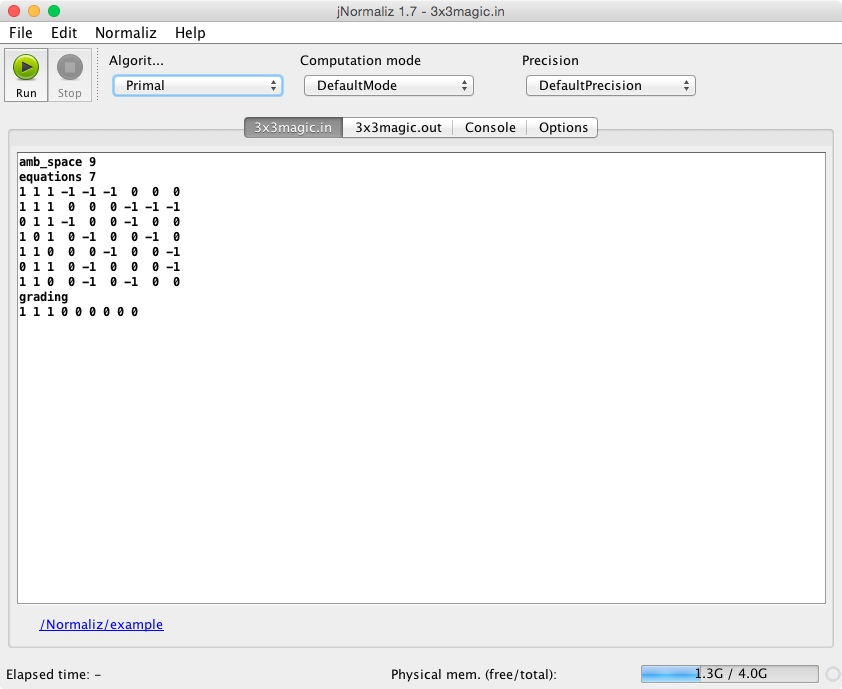
\includegraphics[width = 80 mm, bb=0 0 690 560]{jNormaliz.jpg}\\%width = 80 mm, bb=0 0 689 430
  \caption{jNormaliz}\label{new}
\end{figure}
In the jNormaliz file dialogue choose one of the input files
in the subdirectory \ttt{example}, say \ttt{small.in}, and
press \ttt{Run}. In the console window you can watch Normaliz
at work. Finally inspect the output window for the results.

The menus and dialogues of jNormaliz are self explanatory, but you
can also consult the documentation \cite{AI} via the help menu.

If the executables prepared cannot be run on your system, then
you can  compile Normaliz yourself (see Section
\ref{Compile}).

Moreover, one can, and often will, run Normaliz from the
command line. This is explained in Section \ref{options}.

If 64 bit integer precision is not sufficient, then one can
switch jNormaliz to infinite precision (or use the option
\texttt{-B} from the command line). Then Normaliz has no
restrictions on the integer precision. See Section
\ref{NumLim}. (The integer precision has nothing to do with the
address width (32 bit or 64 bit) of your operating system.)


%%%%%%%%%%%%%%%%%%%%%%%%%%%%%  INPUT  %%%%%%%%%%%%%%%%%%%%%%%%%%%%%
\section{The input file}\label{input}

The input file \ttt{<project>.in} consists of one or
several matrices. Each matrix is built as follows:

\begin{arab}
\item The first line contains the number of rows $m$.
\item The second contains the number of columns $n$.
\item The next $m$ lines of $n$ integers each contain the rows.
\item The last line contains a single number or word
    specifying the type of input the matrix presents.
\end{arab}

The line structure is irrelevant for the interpretation of the input, and only meant as a suggestion for a transparent structure of the file. The examples below are often typeset in two columns. It should always be obvious how to read them properly.

At the moment there are three major classes of input matrices,
namely \emph{generators}, \emph{constraints}, and
\emph{relations}.

Generators and constraints themselves fall into two subclasses:

\begin{arab}
\item \emph{homogeneous}, defining cones and lattices,
\item \emph{inhomogeneous}, defining polyhedra and affine lattices.
\end{arab}

Additional classes are \emph{grading} and \emph{dehomogenization}.

\emph{Remark}.\enspace Normaliz 2.12 (like Normaliz 2.11) allows inhomogeneous input types. While polytopes are defined by inhomogeneous data, one usually wants to compute the cone over the polytope, its Hilbert basis and the Ehrhart series. These computations require \emph{homogeneous} input types, and their application to polytopes is explained below. Also see Section \ref{po_vs_po}.

Rules for the combination of input types:

\begin{arab}
\item The order of the matrices does not matter.
\item Matrices of the same type will be concatenated (and must have the same number of columns).
\item The three classes generators, constraints and relations exclude each other (at present), with one exception: \verb|excluded_faces| are allowed with homogeneous generators.
\item There can be at most one type of generators.
\item Homogeneous and inhomogeneous constraints can be mixed. As soon as an inhomogeneous type is present, Normaliz treats the input as being inhomogeneous, transforming the homogeneous types appropriately.

Exception: \verb|excluded_faces| are forbidden in combination with inhomogeneous constraints for which they are replaced by \verb|strict_inequalities|.
\end{arab}

For each input type we specify two lattices: the \emph{ambient
lattice} $\AA$ to which the input data refer and the
\emph{essential lattice} $\EE\subset \AA$ with respect to which
all data are computed.

In this section we assume that Normaliz is run in a computation
mode in which the Hilbert basis or the system of generators, respectively, is actually computed. (See Section
\ref{options} for computation modes.)

\subsection{Generators of cones and lattices}

These generator types are \verb|integral_closure|, \verb|normalization|, \verb|polytope| and \verb|rees_algebra|.

\subsubsection{Type \ttt{integral\_closure}}

The rows of an $m\times n$ matrix of this type represent $m$ vectors in
the ambient lattice $\AA=\ZZ^n$. The essential lattice $\EE$ is the
smallest direct summand of $\ZZ^n$ that contains the vectors in the
matrix.

The vectors are considered as a system of generators $\cG$ of a
cone $C$, and Normaliz computes the Hilbert basis of $C$ with
respect to $\EE$ (or, equivalently,  $\ZZ^n$).

The nomenclature \ttt{integral\_closure} is explained by the
fact that the Hilbert basis generates the integral closure of
the monoid $\ZZ_+\cG$ in $\ZZ^n$.

A simple example:

\begin{Verbatim}
Input            Hilbert basis
3                1 0
2                0 1
2 0
1 1
0 2
integral_closure
\end{Verbatim}

In this example, the three input vectors clearly generate the
positive orthant $\RR_+^2$ in $\RR^2$, and the two unit vectors
clearly are the Hilbert basis of $\RR_+^2\cap\ZZ^2$.

Example input files: \ttt{rproj2.in}, \ttt{small.in}.

\subsubsection{Type \ttt{normalization}}\label{normalization}

The matrix is interpreted as as one of type \verb|integral_closure|, however $\EE$ is chosen as
the sublattice of $\ZZ^n$ generated by $\cG$.

The choice of the name \ttt{normalization} indicates that
Normaliz computes the normalization of the monoid $\ZZ_+\cG$.
(The computation of such normalizations was the original goal
of Normaliz, hence the name.)

We choose the same input vectors as above, but change the type to
\ttt{normalization}:

\begin{Verbatim}
Input            Hilbert basis
3                2 0
2                1 1
2 0              0 2
1 1
0 2
normalization
\end{Verbatim}

The cone has not changed, but the lattice has: $\EE$ is now the
sublattice of $\ZZ^2$  of all $(z_1,z_2)$ with $z_1+z_2\equiv 0
\mod 2$.

Example input files: \ttt{rafa2416.in}, \ttt{A443.in}.

\subsubsection{Type \ttt{polytope}}

The rows of the matrix are interpreted as integral points of a
lattice polytope in $\RR^n$, which is their convex hull.

The cone $C$ is the cone over the polytope, i.e.\ the cone with apex
$0$ in $\RR^{n+1}$ generated by the vectors $(x,1)$ where $x$
represents a row of the input matrix. We want to compute the \emph{Ehrhart
monoid} $C\cap \ZZ^{n+1}$.

The lattice $\AA$ is $\ZZ^{n+1}$, and $\EE$ is the smallest
direct summand of $\AA$ containing the generators of $C$.

Type \ttt{polytope} is only a variant of type \verb|integral_closure|. One obtains the same results as
in type \verb|integral_closure| with the extended vectors $(x,1)$ as input.

Example input files: \ttt{polytop.in}, \ttt{FortuneCookie.in},
\ttt{lo6.in}.

\subsubsection{Rational polytopes}\label{rat_pol_in}

Normaliz has no special input type for rational polytopes.
In order to process them one uses type \verb|integral_closure| together with a
grading. Suppose the polytope is given by vertices
$$
v_i=(r_{i1},\dots,r_{in}),\qquad i=1,\dots,m,\ r_{ij}\in\QQ.
$$
Then we write $v_i$ with a common denominator:
$$
v_i=\biggl(\frac{p_{i1}}{q_i},\dots,\frac{p_{in}}{q_i}\biggr),
\quad p_{ij},q_i\in\ZZ,\ q_i>0.
$$
The generator matrix is given by the rows
$$
\widetilde v_i=(p_{i1},\dots,p_{in},q_i),\quad i=1,\dots,m.
$$
We must add a grading since Normaliz cannot recognize it
without help (unless all the $q_i$ are equal). The grading
linear form has coordinates $(0,\dots,0,1)$. See \ref{grading} below
for general information on gradings.

Let us look at a concrete example (contained in \ttt{rational.in}),
the triangle $P$ with vertices
$$
(1/2,1/2),\ (-1/3,-1/3),\ (1/4,-1/2).
$$
In order to apply Normaliz to it one uses the following
input:

\begin{Verbatim}
3                          1
3                          3
1 1 2                      0 0 1
-1 -1 3                    grading
1 -2 4
integral_closure
\end{Verbatim}

The output will be discussed in \ref{rat_pol_out}.

\subsubsection{Type \ttt{rees\_algebra}}

In this type the input vectors are considered as exponent
vectors of the generators of a monomial ideal $I$ in the
polynomial ring $K[X_1,\dots,X_n]$. Normaliz computes the
normalization of the Rees algebra of the ideal $I$ (see
\cite{BH} for the notion of Rees algebra.) This is a monomial
subalgebra of the extended polynomial ring $K[X_1,\dots,X_n,T]$
with an auxiliary variable $T$. Normaliz computes the
exponent vectors in $\ZZ^{n+1}$ of the system of generators.
For an example, see Section \ref{Examples}.

In type \verb|rees_algebra| one has $\AA=\EE=\ZZ^{n+1}$.

Example input file: \ttt{rees.in}.

\subsubsection{Preparation of the generators}

After the coordinate transformation to the lattice $\EE$,
Normaliz divides each generator by the greatest common
divisor of its components. For example, the extreme rays listed
will always be such $\EE$-primitive vectors (re-transformed to
$\AA$ where they may not be primitive).

If a grading is present, the generators will be sorted by
degree in ascending order. If no grading is available, they will be sorted by their $1$-norm in the lattice $\EE$. Those of the same degree will remain
sorted as in the input file (or the result of a previous
computation).

This preparation is also performed if the generators result from a system of constraints.

\subsection{Homogeneous Constraints}

Homogeneous inequalities, equations, and congruences defining the cone and
the lattice are called \emph{homogeneous constraints}. Matrices
representing them are of types 
\verb|equations|, \ttt{inequa\-li\-ties}, \verb|signs|, \verb|congruences| and \verb|excluded_faces|.


In previous versions \verb|inequalities| were called \verb|hyperplanes|. The name is still allowed, but no longer recommended.

The numbers of columns must of
course match: for the ambient lattice $\AA=\ZZ^n$ the matrices of equations and inequalities must have $n$ columns, and matrices of congruences must
have $n+1$ columns. The essential lattice $\EE$ is the smallest sublattice of $\AA$ containing the solutions of the combined systems of constraints.

If there is no matrix of inequalities, then it is assumed that the
user wants to compute the nonnegative solutions of the system
represented by the equations and congruences.

\subsubsection{Type \ttt{inequalities} (formerly \ttt{hyperplanes})}
A row $(\xi_1,\dots,\xi_n)$ of the input matrix of this type represents
an inequality
$$
\xi_1x_1+\dots+\xi_nx_n\ge 0
$$
for the vectors $(x_1,\dots,x_n)$ of $\RR^n$.

Example:

\begin{Verbatim}
Input            Hilbert basis
2                0 -1
2                1  1
1 0
1 -1
inequalities
\end{Verbatim}

Normaliz has computed the Hilbert basis of the cone defined
by the inequalities $x_1\ge 0$ and $x_1-x_2\ge 0$ with respect
to the lattice $\ZZ^2$.

Example input file: \ttt{Condorcet.in}.

Remark: In previous versions this type was called \verb|hyperplanes|, a name that can still be used.

\subsubsection{Sign inequalities: \ttt{signs}}

There is a shortcut for the  input of inequalities $x_i\ge 0$
or $x_i\le 0$. The input matrix of type \ttt{signs} has format
$1\times n$ and the entries of its single row are in
$\{-1,0,1\}$:
\begin{itemize}
\item[$-1$] stands for $x_i\le 0$,
\item[$1$] stands for $x_i\ge 0$,
\item[$0$] indicates that the sign of $x_i$ is not
    restricted.
\end{itemize}

Example:

\begin{Verbatim}
1
4
1 -1 0 1
signs
\end{Verbatim}

In this example we require that $x_1,x_4\ge 0$ and $x_2\le 0$.

Example input file: \ttt{Condorcet.in}.

\subsubsection{Polytopes by inequalities}
Normaliz has no special input type for polytopes defined by
inequalities since they can easily be specified via type \verb|inequalities|.
Suppose the polytope is given by inequalities
$$
\alpha_{i1}x_1+\dots+\alpha_{in}x_n\ge \beta_i,\quad i=1,\dots,m,\ \alpha_{ij},\beta_i\in \ZZ.
$$
Then we homogenize the inequalities in the form
$$
\alpha_{i1}x_1+\dots+\alpha_{in}x_n-\beta_ix_{n+1}\ge0,
$$
and use type \verb|inequalities| for them in connection with the grading $(0,\dots,0,1)$.

The file \ttt{poly\_ineq.in} contains

\begin{Verbatim}
3
3                          1
2  7 3                     3
-8 2 3                     0 0 1
1 -1 0                     grading
hyperplanes
\end{Verbatim}

It reproduces the triangle that we have discussed in
\ref{rat_pol_in}.

\subsubsection{Type \ttt{equations}}

A row $(\xi_1,\dots,\xi_n)$ of the input matrix of this type represents
an equation
$$
\xi_1x_1+\dots+\xi_nx_n=0
$$
for the vectors $(x_1,\dots,x_n)$ of $\RR^n$.

Example:

\begin{Verbatim}
Input            Hilbert basis
1                2 0 1
3                0 2 1
1 1 -2           1 1 1
equations
\end{Verbatim}

If the input file contains no further matrices, Normaliz has
computed the Hilbert basis of the subcone of $\RR_+^3$ defined
by the equation $x_1+x_1-2x_3= 0$.

Example input files: \ttt{4x4.in}, \ttt{5x5.in}.

\subsubsection{Type \ttt{congruences}}

We consider the rows of a matrix of this type to have length $n+1$.
Each row $(\xi_1,\dots,\xi_n,c)$ represents a congruence
$$
\xi_1z_1+\dots+\xi_nz_n\equiv 0 \mod c
$$
for the elements $(z_1,\dots,z_n)\in\ZZ^n$.

Example:

\begin{Verbatim}
Input            Hilbert basis
1                2 0
3                1 1
1 1 2            0 2
congruences
\end{Verbatim}

If no other matrix is in the input file, then Normaliz
computes the Hilbert basis of the positive orthant intersected
with the lattice of all integral vectors $(z_1,z_2)$ such that
$z_1+z_2\equiv 0 \mod 2$ and the result is the same as in
\ref{normalization} above.

Example input file: \ttt{3x3magiceven.in}.

\subsubsection{Type \ttt{excluded\_faces}}

This type is useful for the computation of Hilbert series of semiopen cones. It is interpreted as follows:

\begin{arab}
\item If used with input of type \emph{generators}, the faces defined by \verb|excluded_faces| are simply excluded. They do \emph{not} restrict the cone.
\item Otherwise \verb|excluded_faces| has a twofold meaning: (a) they are additional inequalities defining the cone; (b) the faces they define are excluded from the Hilbert series computation.
\end{arab}
The twofold interpretation in case (b) saves the user from including the \verb|excluded_faces| twice.

An example of type (a):
\begin{Verbatim}
4                       1
2                       3
0 0                     1 1 0
0 1                     excluded_faces
1 1
1 0
polytope
\end{Verbatim}


defines the unit square in $\RR^2$, but $(0,0)$ excluded from the Hilbert series computation (See Section \ref{ex_fac_out} for the discussion of the output.)


An example that combines \verb|excluded_faces| with other constraints:
\begin{Verbatim}
1 24
1 1 1 1 1 1 1 1 1 1 1 1 1 1 1 1 1 1 1 1 1 1 1
signs
3 24
1 1 1 1 1 1 -1 -1 -1 -1 -1 -1 1 1 -1 -1 1 -1 1 1 -1 -1 1 -1
1 1 1 1 1 1 1 1 -1 -1 1 -1 -1 -1 -1 -1 -1 -1 1 1 1 -1 -1 -1
1 1 1 1 1 1 1 1 1 -1 -1 -1 1 1 1 -1 -1 -1 -1 -1 -1 -1 -1 -1
excluded_faces
\end{Verbatim}
The semiopen cone described by this input is the intersection of the positive orthant in $\RR^{24}$ with $3$ halfspaces that are defined by the linear forms given as \verb|excluded_faces|, and the facets defined by these linear forms are then excluded.

Note that \verb|excluded_faces| only affect the Hilbert series. They are ignored for all other computations.

Example input file: \ttt{SquareMinusVertex.in, CondParSemi.in}.

\subsubsection{The constraints combined}

Let $L$ be the sublattice of $\ZZ^n$ that consists of the
solutions of the system of congruences defined by the input
matrix of type \ttt{congruences}. ($L=\ZZ^n$ if there is no
such matrix.) Moreover, let $A$ be the matrix of type
\ttt{inequalities}  (combined with the matrix representing the
\ttt{signs}) and $B$ be the matrix of type \ttt{equations}.
Then the cone $C$ is given by
$$
C=\{x\in\RR^n: Ax\ge 0,\ Bx= 0\},
$$
and the Hilbert basis of $C\cap L$ is computed.

The ambient lattice $\AA$ is $\ZZ^n$, and the essential lattice
is $\EE=L\cap \RR C$.

If there is no matrix of type \ttt{equations}, then the system
of equations is empty, satisfied by all vectors of $\RR^n$.

If the input is of type constraints and there are no explicit inequalities contained in it, then Normaliz adds the $n\times n$ unit matrix of \verb|inequalities| to restrict all computations to the nonnegative orthant.

See Section \ref{magiceven} for an example combining types
\ttt{equations} and \ttt{congruences}.

Example input file: \ttt{3x3magiceven.in}.


\subsection{Relations}\label{relations}

Relations do not select a
sublattice of $\ZZ^n$ or a subcone of $\RR^n$, but define a
monoid as a quotient of $\ZZ_+^n$ modulo a system of
congruences (in the semigroup sense!).

The rows of the input matrix of this type are interpreted as
generators of a subgroup $U\subset\ZZ^n$, and Normaliz computes an affine monoid and its normalization  as explained in Section \ref{binomials}.

Set $G=\ZZ^n/U$ and $L=G/\textup{torsion}(G)$. Then the ambient lattice
is $\AA=\ZZ^r$, $r=\rank U$, and the essential lattice is $L$, realized
as a sublattice of $\AA$. Normaliz computes the image of $\ZZ^n_+$ in $L$ and its normalization.

\subsubsection{Type \ttt{lattice\_ideal}}

As an example we consider the binomials $X_1X_3-X_2^2$,
$X_1X_4-X_2X_3$:

\begin{Verbatim}
Input            Hilbert basis
2                3 0
4                2 1
1 -2  1 0        1 2
1 -1 -1 1        0 3
lattice_ideal
\end{Verbatim}

In this example $\ZZ^4/U$ is torsionfree, but we can replace each
of the vectors in the input matrix by a nonzero integral
multiple without changing the result.

The type \ttt{lattice\_ideal} cannot be combined with any other input type (except
\ttt{grading})---such a combination would not make sense. (See Section \ref{grad_lattid} for the use of a grading in this case.)

Example input file: \ttt{lattice\_ideal.in}.

\subsection{Generators of polyhedra}

\subsubsection{Type polyhedron}

A matrix of type polyhedron contains both the generators of the recession cone $C$ and (a superset of) the vertices of the polyhedron. For a polyhedron in $\RR^n$ the vectors have $n+1$ entries in $\ZZ$. The last component must be nonnegative. It is interpreted as follows:
\begin{arab}
\item If it is $0$, the vector is part of the system of generators of $C$.
\item If it is a positive integer, it is considered as the denominator for the first $n$ entries, which together define a (potential) vertex of $P$ in $\QQ^n$.
\end{arab}
The order of the input vectors is irrelevant.
\begin{Verbatim}
4 3
1 0 0
0 1 0
3 2 2
2 3 2
polyhedron
\end{Verbatim}
defines the polyhedron
$$
P=\conv((3/2,1),\ (1,3/2))+\RR_+^2
$$
in $\RR^2$.

Presently there is no possibility  to restrict the lattice. If a polyhedron $P\subset\RR^n$ is defined by a matrix of type \verb|polyhedron|, then all lattice related computations will refer to the standard lattice $\ZZ^n$. Therefore $\AA=\EE=\ZZ^n$ for this input type.

Example input file: \verb|polyhedron.in|

Remark: For computations of (rational)  polytopes (i.e., bounded polyhedra) you almost always want to use the input types \verb|polytope| or \verb|integral_closure| (in conjunction with a grading). We discuss this point in Section \ref{po_vs_po}.

\subsection{Inhomogeneous constraints}

What has been said about homogeneous constraints holds analogously for inhomogeneous ones. Note that we must accommodate a right hand side in inhomogeneous constraints, and therefore inhomogeneous constraints are one component longer than their homogeneous counterparts (with the exception of \verb|strict_inequalities| and \verb|strict_signs|).

If there are no explicit inequalities in the input, then, as in the homogeneous case, it is assumed that nonnegative solutions are to be computed.

The lattice $\EE$ for the computation of the recession module is the sublattice of solutions of the homogeneous constraints associated to the given inhomogeneous constraints. (So it is defined even if the polyhedron is empty.) The affine lattice for the computation of lattice points in the polyhedron is the set of solutions of the given system of constraints.

\subsubsection{Type \ttt{inhom\_inequalities}}

We consider inequalities
$$
\xi_1x_1+\dots+\xi_nx_n\ge \eta, \qquad \xi_i,\eta\in\ZZ,
$$
rewritten as
$$
\xi_1x_1+\dots+\xi_nx_n+(-\eta) \ge 0
$$
and then represented by the input vector
$$
(\xi_1,\dots,\xi_n,-\eta).
$$
\begin{Verbatim}
2
3
1 0 -1
0 1 -2
inhom_inequalities
\end{Verbatim}
describes the polyhedron
$$
P=\{x\in\RR^2: x_1\ge1,x_2\ge2\}.
$$

Remark: For computations of (rational)  polytopes (i.e., bounded polyhedra) you almost always want to use the input type \verb|inequalities|. We discuss this point in Section \ref{po_vs_po}.

Example input file: \verb|SquareMinusVertexInhom.in, NonCMDivisor.in|.

\subsubsection{Type \ttt{strict\_inequalities}}
These are shortcuts for inequalities of type
$$
\xi_1x_1+\dots+\xi_nx_n\ge1.
$$
\begin{Verbatim}
2
2
1 0
0 1
strict_inequalities
\end{Verbatim}
describes the polyhedron
$$
P=\{x\in\RR^2: x_1\ge1,x_2\ge1\}.
$$

Example input file: \verb|CondorcetInt.in|.

\subsubsection{Type \ttt{strict\_signs}}

The components of a (one rowed) matrix of this type are interpreted as follows:
\begin{itemize}
\item[$-1$] stands for $x_i\le -1$,
\item[$1$] stands for $x_i\ge 1$,
\item[$0$] indicates that $x_i$ is not
    restricted.
\end{itemize}
\begin{Verbatim}
1
3
1 -1 1
strict_signs
\end{Verbatim}
represents the inequalities
$$
x_1\ge 1,\ x_2\le-1,\ x_3\ge1.
$$

Example input file: \verb|CondorcetInt.in|.

\subsubsection{Type \ttt{inhom\_equations}}
We consider equations
$$
\xi_1x_1+\dots+\xi_nx_n= \eta, \qquad \xi_i,\eta\in\ZZ,
$$
rewritten as
$$
\xi_1x_1+\dots+\xi_nx_n+(-\eta) = 0
$$
and then represented by the input vector
$$
\xi_1,\dots,\xi_n,-\eta.
$$
The input
\begin{Verbatim}
2
4
1 2 3 -2
3 2 -2 5
inhom_equations
\end{Verbatim}
represents the system
\begin{align*}
x_1+2x_2+3x_3&=2,\\
3x_1+2x_2-2x_3&=-5.
\end{align*}

Example input file: \verb|InhomIneq.in|.

\subsubsection{Type \ttt{inhom\_congruences}}
We consider the rows of a matrix of type \verb|inhom_congrueneces| to have length $n+2$.
Each row $(\xi_1,\dots,\xi_n,-\eta,c)$ represents a congruence
$$
\xi_1z_1+\dots+\xi_nz_n\equiv \eta \mod c
$$
for the elements $(z_1,\dots,z_n)\in\ZZ^n$.
\begin{Verbatim}
2
4
1 2 -3 7
2 2 -4 13
inhom_congrueneces
\end{Verbatim}
represents the system
\begin{align*}
 x_1 + 2x_2 &\equiv 3\pod 7,\\
2x_2 +  x_2 &\equiv 4\pod{13}
\end{align*}
of simultaneous congruences.

Example file: \verb|ChineseRemainder.in|.

\subsubsection{Mixing homogeneous and inhomogeneous constraints}

Homogeneous and inhomogeneous constraints can appear in the same input file. Note that there must be at least one inhomogeneous type in order to indicate to Normaliz that the input is inhomogeneous.

The homogeneous constraints will simply be considered as inhomogeneous constraints with right hand side $0$. An example:
\begin{Verbatim}
2                           1
4                           3
0 1 0 -1                    1 0 0
0 0 1 -1                    inequalities
inhom_inequalities
\end{Verbatim}
defines the polyhedron
$$
P=\{x\in\RR^3: x_1\ge0, x_2\ge1, x_3\ge1\}.
$$

\subsection{Grading}\label{grading}

$\ZZ$-valued grading can be specified in two ways:
\begin{arab}
\item \emph{explicitly} by including a grading in the input, or
\item \emph{implicitly}. In this case Normaliz checks whether
    the extreme integral generators of the monoid lie in an
    (affine) hyperplane $A$. If so, then the (unique) primitive
    $\ZZ$-linear form $\lambda$ that affords an equation
    $\lambda(x)=b$ for $A$ is used as the grading.
\end{arab}



\emph{Note:} In previous versions we used \emph{height} as a
synonym for \emph{degree}.

A grading is explicitly specified by an $1\times n$ matrix for
cones embedded in $\RR^n$, and its type is fixed by the
attribute \ttt{grading}, for example

\begin{Verbatim}
1
2
3 2
grading
\end{Verbatim}

Normaliz checks whether all generators of the monoid have
positive degree.

Before Normaliz can apply the degree, it must be restricted
to the effective lattice $\EE$. Even if the entries of the
grading vector are coprime, it often happens that all degrees
of vectors in $\EE$ are divisible by a greatest common divisor
$ d>1$. Then $d$ is extracted from the degrees, and it will
appear as \ttt{denominator} in the output file.

Special rules apply to some input types that we explain in the
following.

\subsubsection{\ttt{polytope}}
Cones defined by lattice polytopes always have an implicit
grading in which the lattice points in the polytope have degree
$1$ (roughly speaking). Therefore it is not possible to use an
explicit grading together with this input type.

If it should be necessary to apply a different grading, then
one converts the input of type \ttt{polytope} to
\ttt{integral\_closure} by appending \ttt{1} to each row of the
input matrix and adds the grading to be used.

\subsubsection{\ttt{rees\_algebra}} Suppose that the rows of the
input matrix specify vectors of length $n$. Then these are
embedded into $\RR^{n+1}$, and therefore the grading must have
$n+1$ components. Example:

\begin{Verbatim}
3                           1
3                           4
0 1 2                       1 1 1 -1
2 0 2                       grading
1 1 1
rees_algebra
\end{Verbatim}


Note that the Rees algebra has an implicit grading if and only
if all the monomials have the same total degree, say $g$. Then
the grading vector chosen automatically is
$(1,\dots,1,-(g-1))$.

\subsubsection{\ttt{lattice\_ideal}} \label{grad_lattid}

In this case the unit vectors correspond to generators of the
monoid. Therefore the degrees assigned to them must be
positive. Moreover, the vectors in the input represent binomial
relations, and these must be homogeneous. In other words, both
monomials in a binomial must have the same degree. This amounts
to the condition that the input vectors have degree $0$.
Normaliz checks this condition. Example:


\begin{Verbatim}
1 4                        1 4
1 1 -1 -1                   1 2 1 2
lattice_ideal               grading
\end{Verbatim}

\subsubsection{Inhomogeneous input}

Recall that inhomogeneous data defining a polyhedron in $\RR^n$ have length $n+1$ (or even $n+2$ in the case of inhomogeneous congruences). The grading assigns a degree to each of the $n$ canonical basis elements of $\ZZ^n$, and therefore has length $n$:
\begin{Verbatim}
2  3                           1 2
1 1 5                          1 1
1 -1 4                         grading
inhom_inequalities
\end{Verbatim}
is an example of consistent input.

\subsection{Dehomogenization}

Inhomogeneous input for objects in $\RR^d$ is homogenized by an additional coordinate and then computed in $\RR^{d+1}$, but with the additional condition $x_{d+1}\ge 0$, and then dehomogenizing all results: the substitution $x_{d+1}=1$ acts as the \emph{dehomogenization}, and the inhomogeneous input types implicitly choose this dehomogenization.

Like the grading, one can define the dehomogenization explicitly as in the following example:
\begin{Verbatim}
2 3                    1 3
-1 1 0                 1 0 0
-1 0 1                 dehomogenization
inequalities                              
\end{Verbatim}
This input is equivalent to
\begin{Verbatim}
2
3
1 0 -1
0 1 -1
inhom_inequalities
\end{Verbatim}

But the dehomogenization can be any linear form $\delta$  satisfying the condition $\delta(x)\ge 0$ on the cone that is truncated. (In combination with constraints, the condition $\delta(x)\ge 0$ is automatically satisfied since $\delta$ is added to the constraints.)

Since inhomogeneous input defines a dehomogenization implicitly, the type \verb|dehomogenization| cannot be combined with any of the inhomogeneous input types. It is also forbidden for
\begin{center}
 \verb|normalization|, \verb|polytope|, \verb|rees_algebra| and \verb|lattice_ideal|.
\end{center}
(Note that \verb|polytope| defines its own homogenization via the grading by the last coordinate.)

The input type \verb|dehomogenization| makes the computation inhomogeneous, resulting in inhomogeneous output. The polyhedron computed is the intersection of the cone $C$ (and the lattice $L$) defined by the remaining components of the input with the hyperplane given by $\delta(x)=1$, and the recession cone is $C\cap\{x:\delta(x)=0\}$.

A potential application is the adaptation of other input formats like that of polymake to Normaliz. For example, if the first coordinate is used as the homogenizing variable, then the system of inequalities above is given as
\begin{Verbatim}
2                      1
3                      3
-1 1 0                 1 0 0
-1 0 1                 dehomogenization
inequalities                              
\end{Verbatim}

Example input file: \verb|dehomogenization.in|.


\subsection{Pointedness}


For Hilbert basis computations and triangulations Normaliz
requires the (recession) cone to be pointed ($x,-x\in C\implies x=0$).
Whenever the condition of pointedness is violated at a step
where it is crucial, Normaliz will stop computations.

Pointedness is checked by testing whether the dual cone of $C$
is full dimensional, and if not, then the constructor of the
cone complains as follows:

\begin{Verbatim}
Full Cone error: Matrix with rank = number of columns needed in
the constructor of the object Full_Cone. Probable reason: Cone
not full dimensional(<=> dual cone not pointed)!
\end{Verbatim}

\subsection{The zero cone}\label{zero}

The zero cone with an empty Hilbert basis is a legitimate
object for Normaliz. Nevertheless a warning message is issued
if the zero cone is encountered.

\subsection{Additional input file for NmzIntegrate}

NmzIntegrate, whether called by Normaliz or from the command
line, needs an input file \ttt{<project>.pnm} that contains
the polynomial for which the generalized Ehrhart series or the
integral is to be computed. See \cite{NmzInt}.

\subsection{Number codes for input types}

For historical reasons some of the input types can be represented by numbers instead of names. We strongly advise the user to avoid them now despite that they can still be used. These codes are

\begin{enumerate}
\item[0:] \verb|integral_closure|
\item[1:] \verb|normalization|
\item[2:] \verb|polytope|
\item[3:] \verb|rees_algebra|
\item[4:] \verb|inequalties| (or \verb|hyperplanes|)
\item[5:] \verb|equations|
\item[6:] \verb|congruences|
\item[10:] \verb|lattice_ideal|
\end{enumerate}

%%%%%%%%%%%%%%%%%%%%%%%%%%%%%  RUNNING  %%%%%%%%%%%%%%%%%%%%%%%%%%%%%
\section{Running Normaliz}\label{options}

The simplest way to call Normaliz from the command line is
\begin{center}
\ttt{normaliz <project>}
\end{center}
for example
\begin{center}
\ttt{normaliz rafa2416}
\end{center}
The project name is \ttt{rafa2416}. Normaliz reads the input
file \ttt{rafa2416.in} (hopefully existing), computes
everything it can compute, and writes the output to
\ttt{rafa2416.out}.  (We assume
that the executable \ttt{normaliz} or \ttt{normaliz.exe} is in the
search path. Otherwise you have to prefix it with a suitable
relative or absolute path.)

In the following we explain the various options of Normaliz.
The full text names given appear in the help screen as well as
in the menus of jNormaliz which allows you to choose options
interactively.

{\bf In the default computation mode Normaliz will try to compute all data
accessible to it, using the triangulation based \emph{primal} algorithm. All
options that
can be activated are switched off by default.}

The default mode is broken by any option that asks for a specific computation. These are all \emph{except}
\begin{center}
\ttt{ceBfax}.
\end{center}
\subsection{Full syntax and basic rules}

The full syntax for calling Normaliz from the command line is
\begin{center}
\hspace*{-1cm}\ttt{normaliz [-sN1vq]  [-nph] [-dr] [-tTy] [-ceB] [-fa] [-ELI] [-x=<T>] [<project>]}
\end{center}
where the options and \ttt{<project>} are optional.

A help screen can be displayed by \ttt{normaliz -?}.

Basic rules for the use of options:

\begin{enumerate}
\item If no \ttt{<project>} is given, the
program will ask you for it or display a help screen.

\item The option \ttt{-x} differs from the other ones: \ttt{<T>}
represents a positive number assigned to \ttt{-x}; see
Section \ref{exec}.

\item Normaliz will look for \ttt{<project>.in} as input
file.

If you inadvertently typed \ttt{rafa2416.in} as the project
name, then Normaliz will first look for \ttt{rafa2416.in.in}
as the input file. If this file doesn't exist,
\ttt{rafa2416.in} will be loaded.

\item Adding a pure output option, namely \ttt{-f} or \ttt{-a}, or an
option controlling execution does not change the computation
mode. In particular, it does not change the default computation mode.

\item The options can be given in arbitrary order. All options are accumulated,
and there is no mutual exclusion.

\item However, not all options are allowed for inhomogeneous input data; see
Section \ref{OptInhom}.

\item If Normaliz cannot perform a computation explicitly asked for by the
user, it will terminate. Typically this happens if no grading is given although
it is necessary.

\item In the default mode Normaliz does not complain about missing data
(anymore). It will simply omit those computations that are impossible.

\item If a certain type of computation is not asked for explicitly, but can
painlessly be produced as a side effect, Normaliz will compute it. For
example, as soon as a grading is present and the Hilbert basis is computed, the
degree $1$ elements of the Hilbert basis are selected from it.

\end{enumerate}

For example, if you input the command
\begin{center}
\ttt{normaliz -c -p -a rafa2416 -T -y}\qquad or\qquad
\ttt{normaliz -cpaTy rafa2416}
\end{center}
then the program will take the file \ttt{rafa2416.in} as input,
control data will be displayed on your terminal, the support
hyperplanes, the triangulation, the multiplicity, the Hilbert
series and the Hilbert (quasi)polynomial will be computed and
all the possible output files will be produced.

\subsection{Computation modes: homogeneous input}

\subsubsection{Basic modes}

The least that Normaliz can do is
\begin{itemize}
\itemtt[-s] \ttt{support hyperplanes}: only the constraints  of the cone and the lattice  under consideration and the
    extreme rays are computed.
\end{itemize}
All computation modes include \ttt{-s}.

For Hilbert basis computations one uses
\begin{itemize}
\itemtt[-N] \ttt{Hilbert basis}: computes the Hilbert basis.
\end{itemize}
The degree $1$ elements of the Hilbert basis are computed by
\begin{itemize}
\item [-1] \ttt{degree 1 elements}: only degree 1 elements are computed.
\end{itemize}

Enumerative data are chosen by
\begin{itemize}
\itemtt[-v] \ttt{volume}: Normaliz
    computes the multiplicity (or normalized volume);
\itemtt[-q] \ttt{Hilbert series}.
\end{itemize}

Remarks: (1) The Hilbert basis can also be computed by the dual algorithm; see
Section \ref{dual}. In the presence of a grading, \ttt{-N} includes the
computation of the degree $1$ elements.

(2) For degree $1$ elements the dual algorithm can be applied as well.
Moreover, the approximation of rational polytopes is available for this
purpose; see Section \ref{approx}.

(3) The options \ttt{-1vq} require the presence of a grading (implicit or explicit).

(4) \ttt{-N} and \ttt{-1} only need a partial triangulation, whereas the options \ttt{-vq}
require a full triangulation.

\subsubsection{Combined modes}

For convenience, Normaliz provides shortcut modes that combine basic modes:

\begin{itemize}
\itemtt[-n] \ttt{Hilbert basis volume}: combines \ttt{-N} and \ttt{-v};
\itemtt[-p] \ttt{Hilbert series degree 1 elements}.This mode
    combines \ttt{-q} and \ttt{-1};
\itemtt[-h] \ttt{Hilbert basis series}: combines \ttt{-N} and \ttt{-q}. This
    computation mode yields the maximum information Normaliz can produce.
\end{itemize}

Remarks: (1) There is no mode combining \ttt{-v} and \ttt{-1}. Simply use
\ttt{-v1}.

(2) The effect of \ttt{-h} is also reached by the default mode. However,
\ttt{-h} will result in termination if a grading cannot be found.

\subsubsection{The dual algorithm}\label{dual}

If a cone is defined by constraints, it is often (but not
always) faster to use a Hilbert basis algorithm originally due
to Pottier \cite{Po} that we call the \emph{dual} algorithm, in
contrast to the primal (triangulation based) algorithm
of Normaliz. (See \cite{BI} for our version of the dual
algorithm.) The dual algorithm is invoked by

\begin{itemize}
\itemtt[-d] \ttt{dual Hilbert basis}: computes the Hilbert basis using the
dual algorithm;

\itemtt[-d1] \ttt{dual degree 1}: computes only the degree $1$ elements.
\end{itemize}

Remarks: (1) The dual algorithm can be used with all input types. See
Section \ref{PerPar} for a comparison of performance on various
examples.

(2) \ttt{-d1} is optimized for the computation of degree $1$ elements.

(3) The dual algorithm can be combined with the primal algorithm. For example,
\ttt{-d1v} or \ttt{-dq} make perfect sense, and are often useful.

(4) If \ttt{-d} is set, the dual algorithm has priority in the computation of
Hilbert bases, but not necessarily in the computation of degree $1$ elements.
For example, \ttt{-d1q} will bypass the dual algorithm, since the degree $1$
elements can be gotten as a byproduct of \ttt{-q}.

\subsubsection{Approximation of rational polytopes}\label{approx}

Even the computation of degree $1$ elements can be an extremely difficult
problem in the primal as well as in the dual approach. A major obstruction in
the primal algorithm is the occurrence of gigantic determinants of the
simplicial cones in the triangulation. In this case the approximation of a
rational polytope by a lattice polytope offers a way out:

\begin{itemize}
\itemtt[-r] \ttt{approximate rat polytope}: computes the lattice points in the
degree $1$ cross-section by approximation.
\end{itemize}

It makes no sense to combine \ttt{-r} with the computation of a Hilbert basis
or Hilbert series or with the dual mode. In such case \ttt{-r} is bypassed.
However, \ttt{-rv} makes sense.

\subsubsection{What option do I use \dots}

The following table gives an overview of the computation
options introduced so far.
\begin{center}
\begin{tabular}{l|c|c|c|}
&No enumera-&&Hilbert\\
&tive data&multiplicity&series\\
\hline
only extreme&&&\\
rays&\ttt{-s}&\ttt{-v}&\ttt{-q}\\
\hline
degree 1&\ttt{-1}&\ttt{-v1}&\\
elements &\ttt{-d1, -r}&\ttt{-d1v, -rv}&\ttt{-p}\\
\hline
Hilbert &\ttt{-d}&\ttt{-dv}&default,\\
basis &\ttt{-N}&\ttt{-n}&\ttt{-h, -dq}\\
\hline
\end{tabular}
\end{center}


\subsubsection{Modes calling NmzIntegrate}

NmzIntegrate is an independent executable, but it can be
called by Normaliz. The options are exactly those that would
be used for a command line call of NmzIntegrate:

\begin{itemize}
\itemtt[-E] \ttt{Generalized Ehrhart series}: computation
    of generalized Ehrhart series,
\itemtt[-L] \ttt{Leading coefficient}: computation of
    leading coefficient of generalized Ehrhart
    quasi\-po\-lynomial,
    \itemtt[-I] \ttt{Integral}: computation of Lebesgue
        integrals.
\end{itemize}

See \cite{NmzInt} for the details of NmzIntegrate. The
options \ttt{-c} and \ttt{-x=<T>} are forwarded to
NmzIntegrate.

The option \ttt{-E} contains \ttt{-y}, and \ttt{-I} and
\ttt{-L} both contain \ttt{-T}. See Section \ref{TriStan}
for \ttt{-T} and \ttt{-y}.

Note: the option \verb|-F| of NmzIntegrate cannot be accessed via Normaliz.

\subsubsection{Triangulation and Stanley decomposition}\label{TriStan}

In some applications it may be useful to base further computations on the
triangulation or even the Stanley decomposition computed by Normaliz. As
already mentioned, NmzIntegrate needs these data:
\begin{itemize}
\itemtt[-T] computes the triangulation and writes it to the file
\ttt{<project>.tri}.

\itemtt[-y] computes the Stanley decomposition and writes it to the file
\ttt{<project>.dec}.
\end{itemize}

Both modes generate further output files, namely \ttt{<project.>inv} and
\ttt{<project>.tgn}. The
format of these files will be explained in Section
\ref{optionaloutput}.

There is a further mode computing the triangulation, but producing no output:
\begin{itemize}
\itemtt[-t] Computes the triangulation.
\end{itemize}
Why this option is sometimes useful will be explained in Section \ref{Large}.

\subsection{Computation modes: inhomogeneous input}\label{OptInhom}

The following options are \emph{not allowed} for inhomogeneous input:
\begin{center}
\ttt{1prTyELI}
\end{center}
The other modes are completely analogous to those for cones when one replaces
``Hilbert basis'' by ``system of generators and Hilbert basis of recession monoid'' (see Section \ref{latt_hedra}).
Whether Normaliz computes a cone or a polyhedron does only depend on the
input file and not on the command line options. In order to keep jNormaliz
simple, the same full text names of the options are used for polyhedra.

\subsubsection{Basic modes}

\begin{itemize}
\itemtt[-s] \ttt{support hyperplanes}: only the constraints of the polyhedron and its vertices are computed.
\end{itemize}
All computation modes include \ttt{-s}.

\begin{itemize}
\itemtt[-N] \ttt{Hilbert basis}: computes the system of generators, namely the
Hilbert basis of the recession cone and the minimal system of module generators.
\itemtt[-v] \ttt{volume}: Normaliz computes the multiplicity.
\itemtt[-q] \ttt{Hilbert series}: what it says.
\end{itemize}

Remarks: (1) Systems of generators can also be computed by the dual algorithm;
see Section \ref{dual}.

(2) The options \ttt{-vq} require the presence of a grading.

(3) \ttt{-N} only needs a partial triangulation, whereas the options \ttt{-vq}
require a full triangulation.

\subsubsection{Combination modes}

\begin{itemize}
\itemtt[-n] \ttt{Hilbert basis volume}: combines \ttt{-N} and \ttt{-v};
\itemtt[-h] \ttt{Hilbert basis series}: combines \ttt{-N} and \ttt{-q}. This
    computation mode yields the maximum information Normaliz can produce.
\end{itemize}

The effect of \ttt{-h} is also reached by the default mode. However,
\ttt{-h} will result in termination if a grading cannot be found.

\subsubsection{The dual algorithm}

\begin{itemize}
\itemtt[-d] \ttt{dual Hilbert basis}: computes the system of generators using
the
dual algorithm.
\end{itemize}

\subsubsection{What option do I use \dots}

The following table gives an overview of the computation
options introduced so far.
\begin{center}
\begin{tabular}{l|c|c|c|}
&No enumera-&&Hilbert\\
&tive data&multiplicity&series\\
\hline
only vertices&\ttt{-s}&\ttt{-v}&\ttt{-q}\\
\hline
Hilbert &\ttt{-d}&\ttt{-dv}&default,\\
basis &\ttt{-N}&\ttt{-n}&\ttt{-h, -dq}\\
\hline
\end{tabular}
\end{center}

\subsection{Control of output files}\label{outcontrol}

In the default setting Normaliz writes only the output file
\ttt{<project>.out} (and the files produced by \ttt{-T} and \ttt{-y}). The
amount of output files can be
increased as follows:
\begin{itemize}
\itemtt[-f] Normaliz writes the additional output files
    with suffixes \ttt{gen}, \ttt{cst}, and \ttt{inv},
    provided the data of these files have been computed.
\itemtt[-a] includes \ttt{-f}, Normaliz writes all
    available output files except the triangulation or the
    Stanley decomposition.
\end{itemize}
In order to see all available output files one uses \ttt{-aTy}.

The triangulation and the Stanley decomposition are treated
separately since they can become very large and may exhaust
memory if they must be stored for output.

For the list of potential output files and their interpretation
see Section \ref{optionaloutput}.


\subsection{Control of execution}\label{exec}

The options that control the execution are:

\begin{itemize}
\itemtt[-c] activates the verbose (``console'') behavior of
    Normaliz in which Normaliz writes additional
    information about its current activities to the
    standard output.
\itemtt[-e] activates the overflow error check of
    Normaliz. Ignored if used with -B.
\itemtt[-B] switches Normaliz to infinite precision.
\itemtt[-x=<T>] Here \ttt{<T>} stands for a positive
    integer limiting the number of threads that Normaliz
    is allowed access on your system. The default value is
    set by the operating system. If you want to run
    Normaliz in a strictly serial mode, choose
    \ttt{-x=1}.
\end{itemize}

The number of threads can also be controlled by the environment
variable \verb+OMP_NUM_THREADS+. See Section \ref{PerPar} for
further discussion.

\subsection{Numerical limitations}\label{NumLim}

Even in low dimensions, the range of 64 bit integers may not be
sufficient for the computations of Normaliz. Therefore
\texttt{normaliz} can be switched to infinite precision by the
option \texttt{-B}.

Computations with \ttt{-B} typically run about 5 times slower than
those without it. In examples that look critical, it may be useful
first to try \ttt{normaliz} without \texttt{-B}, but with the error
check option activated. This costs time, too, but hardly more than
50\% extra.

The user should run the example \ttt{critical64.in} in the
subdirectory \ttt{examples} with \ttt{normaliz -e} in order to
see the failure of 64 bit arithmetic. (Running it with \ttt{-B}
takes a while and requires much memory.)

\subsection{Obsolete options}

The options \ttt{-i} and \ttt{-m} of version 2.2 have become
obsolete. They will be ignored if present.

The options \texttt{-SVHP} of versions 2.5 and 2.7 are now
synonymous with\texttt{-svhp} and can still be used.




%%%%%%%%%%%%%%%%%%%%%%%%%%%%%  OUTPUT  %%%%%%%%%%%%%%%%%%%%%%%%%%%%%
\section{The output file}\label{output}

The data you will find in the output file \ttt{<project>.out} depend on the input
type and on the computation mode. The output file starts with
an ``abstract'' that collects various numerical and qualitative
data, for example the number of elements in the Hilbert basis.
The lists of vectors, equations etc.\ follow the abstract.

Note that the values of results computed by Normaliz depend only on the input file, except that the order of vectors in lists like the Hilbert basis can vary, for example because of the unpredictability of the parallelization. The command line parameters only determine which results are computed and what algorithm is used.


\subsection{The homogeneous case}
The output file will contain the following data as far as computed:

\begin{itemize}
\item only for type \verb|lattice_ideal|: the original system of generators
    (see below);
\item  the Hilbert basis $H$ computed;
\item the extreme rays of the cone $C$ generated by $H$;
\item the rank of the lattice $\EE$;
\item the embedding dimension (the rank of $\AA$);
\item the index of the lattice generated by the original input vectors in $\EE$;
\item the support hyperplanes of $C$;
\item a system of equations defining the vector space generated by
$C$;
\item a system of congruences defining $\EE$ as a sublattice of
$\AA$ (together with the equations);
\item the number of simplicial cones in the triangulation
    and the sum of the absolute values of their
    determinants.
\end{itemize}
In the presence of a grading the following extra data may be
printed:
\begin{itemize}
\item the linear form defining the degree;
\item the degree $1$ elements of the Hilbert basis;
\item the multiplicity;
\item the Hilbert series and the coefficients of the
    Hilbert (quasi)polynomial;
\item the excluded faces (if any).
\end{itemize}

The degrees of the extreme rays are listed in the abstract. If
the whole Hilbert basis is of degree 1, this fact is indicated.
Moreover, Normaliz tells you whether the original system of
generators contains the Hilbert basis by indicating whether the
original monoid is integrally closed.

Please note:

\begin{arab}
\item The equations and support hyperplanes \emph{together}
    define the cone $C$. While support hyperplanes will
    always be present (except for the zero cone), equations will
    only be printed if necessary, namely when $\dim
    C<\rank\AA$.

Similarly, congruences will only be printed if the lattice $\EE$
is not given by $\RR C\cap \AA$. This can only happen with
input matrices of types \verb|normalization| or \verb|congruences|.

Even if the cone and the lattice are defined by constraints,
the inequalities, equations and congruences of the input will
in general not be reproduced, but replaced by an equivalent
system.

\item The extreme rays are given by the first points in $\EE$ on
them (the extreme integral generators with respect to $\EE$).

\item In order to lift the grading from
    $\EE$ to $\AA$ it may be necessary to replace it by a
    multiple (in order to avoid fractions as coefficients).
    The necessary factor appears as ``denominator''. The Hilbert series
    and the Hilbert (quasi)polynomial do always refer to the degree in $\EE$.

\item Input matrices of type \emph{generators} contain an explicit
    system of generators. For the other types different from \verb|lattice_ideal|  the extreme rays
    computed by Normaliz take their place. For type \verb|lattice_ideal|
    Normaliz first computes the monoid $M$ generated by the
    residue classes of the canonical basis of $\ZZ^n$ (compare
    Section \ref{relations}), and they are considered as the
    original system of generators.
\end{arab}


In type \verb|rees_algebra|, the data in the output file
refer to the integral closure $\Bar{\cR}$ of the Rees algebra.
In addition to what has been mentioned already, the following
data are computed:

\begin{itemize}
\item the generators of the integral closure of the ideal;
\item if the ideal is primary to the irrelevant maximal
    ideal, the multiplicity of the ideal (not to be
    confused with the multiplicity of the monoid).
\end{itemize}

\subsection{The inhomogeneous case}

\textbf{Note:}\enspace All data are presented in \emph{homogenized coordinates}.
For inhomogeneous input types with implicit dehomogenization this means that all vectors with last component $0$ belong to the recession
cone, and those with last component $>0$ represent a rational point in the
polyhedron with denominator given by the last coordinate.
In constraints the last coordinate represents the negative of the right hand side, as in the input.

If the dehomogenization is another coordinate, the interpretation is analogous. If the dehomogenization $\delta$ is not a coordinate, one must compute it by applying the truncating linear form to the vectors given: the denominator is $\delta(x)$ for the points of the polyhedron. Solving the linear equation $\delta(x)=1$ for one coordinate and substituting the result into the constraints, one obtains inhomogeneous versions of the constraints if they should be needed.

In the inhomogeneous case we compute a polyhedron $P$. We can find the following lists of vectors in the output file describing the solution monoid:
\begin{itemize}
\item the dehomogenization,
\item the generators of the solution module,
\item the Hilbert basis of the solution module.
\end{itemize}
The convex-geometric data of the polyhedron are given by:
\begin{itemize}
\item the vertices of the polyhedron (with denominator $\delta(x)$),
\item the extreme rays of the recession cone.
\end{itemize}

The support hyperplanes, equations and congruences have the same meaning as in the homogeneous case: they describe the polyhedron and the affine lattice with respect to which the solution monoid is computed.

The module rank and the rank of the recession monoid are always computed, as well as the affine dimension of the polyhedron $P$.

If a grading is given, then one can also compute
\begin{itemize}
\item the multiplicity of the solution monoid (the suitably normed leading coefficient of the Hilbert (quasi)polynomial),
\item the Hilbert series given as a rational function with numerator and denominator as in the homogeneous case, however modified by
\item a shift, and
\item the Hilbert (quasi)polynomial, provided the period is not too large.
\end{itemize}

The shift corrects the Hilbert series as follows:
$$
H_{\textup{true}}(t)=t^{-\textup{shift}}H_{\textup{computed}}(t).
$$
The Hilbert (quasi)polynomial must be shifted correspondingly:
$$
q_{\textup{true}}(k)=q_{\textup{computed}}(k+\textup{shift}).
$$

At the end we find the system of constraints that defines the polyhedron $P$ and the set of lattice points in it.

The remarks in the homogeneous case apply accordingly.

%%%%%%%%%%%%%%%%%%%%%%%%%%%%%  EXAMPLES  %%%%%%%%%%%%%%%%%%%%%%%%%%%%%
\section{Examples}\label{Examples}

Note that the output you get by running the examples may differ from the one given below in the order of the vectors in lists like the Hilbert basis. 

\subsection{Generators of cones and lattices}

\subsubsection{Type \ttt{integral\_closure}}

The file \ttt{rproj2.in} contains the following:


\begin{Verbatim}
16 7
 1 0 0 0 0 0 0     0 0 0 0 1 0 0     1 0 1 0 1 0 1     0 1 0 1 1 0 1
 0 1 0 0 0 0 0     0 0 0 0 0 1 0     1 0 0 1 0 1 1     0 1 0 0 1 1 1
 0 0 1 0 0 0 0     1 1 1 0 0 0 1     1 0 0 0 1 1 1     0 0 1 1 1 0 1
 0 0 0 1 0 0 0     1 1 0 1 0 0 1     0 1 1 0 0 1 1     0 0 1 1 0 1 1
                                                       integral_closure
\end{Verbatim}


This means that we wish to compute the cone $C$ generated
by the $16$ vectors
$$
(1,0,0,0,0,0,0)\,,\quad (0,1,0,0,0,0,0)\,,\quad \dots\,,\quad
(0,0,1,1,0,1,1)
$$
in $\RR^7$ with respect to the full lattice $\ZZ^7$, as indicated by
the type \verb|integral_closure|. (Actually, the vectors
generate the full lattice so that a replacement of type \verb|integral_closure| by type \verb|normalization|
would not change anything.)

Running \ttt{normaliz} with no option (or option \ttt{-h},
\ttt{Hilbert basis series}) produces the file \ttt{rproj2.out}
which has the following content (partially typeset in 2 or 3
columns):


\begin{Verbatim}
17 Hilbert basis elements                           multiplicity = 72             
16 Hilbert basis elements of degree 1                                             
16 extreme rays                                     Hilbert series:               
24 support hyperplanes                              1 9 31 25 6                   
                                                    denominator with 7 factors:   
embedding dimension = 7                             1: 7                          
rank = 7 (maximal)                                                                
index = 1                                           Hilbert polynomial:           
original monoid is not integrally closed            60 194 284 245 130 41 6       
                                                    with common denominator = 60  
size of triangulation   = 67
resulting sum of |det|s = 72

grading:
1 1 1 1 1 1 -2 

degrees of extreme rays:
1: 16  

Hilbert basis elements are not of degree 1

***********************************************************************

17 Hilbert basis elements:                 24 support hyperplanes:
 0 0 0 0 0 1 0                               0  0  0  1  0  0  0
 0 0 0 0 1 0 0                               0  0  0  0  1  0  0
 0 0 0 1 0 0 0                               0  0  0  0  0  1  0
 0 0 1 0 0 0 0                               0  0  0  0  0  0  1
 0 0 1 1 0 1 1                               0  0  1  0  0  0  0
 0 0 1 1 1 0 1                               0  1  0  0  0  0  0
 0 1 0 0 0 0 0                               0  1  1  0  0  1 -1
 0 1 0 0 1 1 1                               0  1  0  0  1  1 -1
 0 1 0 1 1 0 1                               0  1  0  1  1  0 -1
 0 1 1 0 0 1 1                               0  0  1  1  0  1 -1
 1 0 0 0 0 0 0                               0  1  1  1  1  1 -2
 1 0 0 0 1 1 1                               0  0  1  1  1  0 -1
 1 0 0 1 0 1 1                               1  0  0  0  0  0  0
 1 0 1 0 1 0 1                               1  1  1  1  1  1 -3
 1 1 0 1 0 0 1                               1  0  0  0  1  1 -1
 1 1 1 0 0 0 1                               1  0  0  1  0  1 -1
 1 1 1 1 1 1 2                               1  0  1  0  1  0 -1
                                             1  0  1  1  1  1 -2
16 extreme rays:                             1  1  1  0  0  0 -1
 1 0 0 0 0 0 0                               1  1  1  1  0  1 -2
 0 1 0 0 0 0 0                               1  1  0  1  0  0 -1
 0 0 1 0 0 0 0                               1  1  1  0  1  1 -2
 0 0 0 1 0 0 0                               1  1  1  1  1  0 -2
 0 0 0 0 1 0 0                               1  1  0  1  1  1 -2
 0 0 0 0 0 1 0
 1 1 1 0 0 0 1               16 degree 1 Hilbert basis elements:
 1 1 0 1 0 0 1                0 0 0 0 0 1 0
 1 0 1 0 1 0 1                0 0 0 0 1 0 0
 1 0 0 1 0 1 1                0 0 0 1 0 0 0       0 1 1 0 0 1 1
 1 0 0 0 1 1 1                0 0 1 0 0 0 0       1 0 0 0 0 0 0
 0 1 1 0 0 1 1                0 0 1 1 0 1 1       1 0 0 0 1 1 1
 0 1 0 1 1 0 1                0 0 1 1 1 0 1       1 0 0 1 0 1 1
 0 1 0 0 1 1 1                0 1 0 0 0 0 0       1 0 1 0 1 0 1
 0 0 1 1 1 0 1                0 1 0 0 1 1 1       1 1 0 1 0 0 1
 0 0 1 1 0 1 1                0 1 0 1 1 0 1       1 1 1 0 0 0 1
\end{Verbatim}


From this, we see that there are $17$ elements in the Hilbert
basis, of which 16 are of degree $1$, and $16$ extreme rays,
that the sublattice generated by the input vectors has index
$1$ in $\ZZ^7$, and that the corresponding support hyperplanes
are given by the linear forms $(0,0,0,1,0,0,0)$,
$(0,0,0,0,1,0,0)$, \dots, $(1,1,0,1,1,1,-2)$.

We are also given the information that there is a grading
(defined implicitly) and what it is. The multiplicity  with
respect to this grading is $72$. By definition, the
multiplicity is the $\EE$-normalized volume of the polytope
obtained by intersecting the cone with the hyperplane at degree
$1$.

The degrees of the extreme rays are given in multiset notation:
\begin{quote}
\ttt{1: 16}
\end{quote}
indicates that $16$ extreme rays have degree $1$.
(The input file contains no explicit grading. The implicitly
defined grading requires that all extreme rays have the same
degree, but it need not be $1$ as in this case.)

Since there is a grading, the degree 1 elements of the Hilbert
basis, the Hilbert series and Hilbert polynomial of the monoid
generated by the Hilbert basis are also computed. The Hilbert
series is given as a rational function. Its numerator
polynomial is
$$
1+9t+31t^2+25t^3+6t^4
$$
as we can see from the vector below the heading \ttt{Hilbert
series}. The denominator is given in multiset notation: \ttt{1:
7} specifies the denominator
$$
(1-t^1)^7.
$$
More general cases will be discussed in \ref{rat_pol_out} and
\ref{magiceven} below.

The Hilbert polynomial is given by
$$
P(k)=\frac{60}{60}+\frac{194}{60}k+\frac{284}{60}k^2+\frac{245}{60}k^3
+\frac{130}{60}k^4+\frac{41}{60}k^5+\frac{6}{60}k^6\,.
$$
The Hilbert polynomial gives the number of elements of degree
$k$, starting from degree $0$, as is always the case for normal
monoids. Note that the multiplicity $m$ can also be read from
the leading coefficient $c$ of the Hilbert polynomial:
\begin{equation}
c=\frac m{(r-1)!},\qquad r=\textup{rank},\label{multlead}
\end{equation}
in our case
$$
c=\frac1{10}=\frac{72}{720}.
$$

The lines

\begin{Verbatim}
size of triangulation = 67
resulting sum of |det|s = 72
\end{Verbatim}

give some information about Normaliz' (not so hard) work: It
produced a triangulation of $67$ simplicial cones, and the sum
of the absolute values of the determinants of their generator
matrices is $72$. It is not surprising that this number equals
the multiplicity. This is always the case if only degree $1$
vectors appear in the generator matrix.

We omit an example of type \verb|normalization| since it does not add anything new.

\subsubsection{Type \ttt{polytope}}\label{latt_pol}

The file \ttt{polytop.in}contains

\begin{Verbatim}
 4
 3
 0 0 0
 2 0 0
 0 3 0
 0 0 5
 polytope
\end{Verbatim}


The Ehrhart monoid of the integral polytope with the $4$
vertices
$$
(0,0,0)\,,\quad (2,0,0)\,,\quad (0,3,0)\quad\text{ and }\quad (0,0,5)
$$
in $\RR^3$ is to be computed. (Note the last line, indicating the
polytope type.)

Running \ttt{normaliz} without an option (or option \ttt{-h}) produces the file \ttt{polytop.out}:


\begin{Verbatim}
19 Hilbert basis elements                         multiplicity = 30          
18 Hilbert basis elements of degree 1                                        
4 extreme rays                                    Hilbert series:            
4 support hyperplanes                             1 14 15                    
                                                  denominator with 4 factors:
embedding dimension = 4                           1: 4                       
rank = 4 (maximal)                                                           
index = 30                                        Hilbert polynomial:        
original monoid is not integrally closed          1 4 8 5                    
                                                  with common denominator = 1
size of triangulation   = 1
resulting sum of |det|s = 30

grading:
0 0 0 1 

degrees of extreme rays:
1: 4  

Hilbert basis elements are not of degree 1                         

***********************************************************************

19 Hilbert basis elements:     18 Hilbert basis elements of degree 1:
 0 0 5 1                        0 0 5 1
 0 3 0 1                        0 3 0 1
 ...                            ...
 1 0 2 1                        1 0 2 1
 1 1 0 1                        1 1 0 1
 1 2 4 2

4 extreme rays:                4 support hyperplanes:
 0 0 0 1                        -15 -10  -6  30
 2 0 0 1                          1   0   0   0
 0 3 0 1                          0   1   0   0
 0 0 5 1                          0   0   1   0
\end{Verbatim}


For the polytopal interpretation one must observe that all data
are in homogenized coordinates for which Normaliz has
appended $1$  to the input vectors that (in this case) are the
vertices of the polytope. In the cone produced, the lattice
points of the polytope are of degree $1$. Therefore the $18$
Hilbert basis elements of degree $1$ represent the lattice
points of the polytope, starting from $(0,0,5)$ and ending with
$(1,1,0)$. The extreme rays represent the $4$ vertices.

From the fact that there are $19$ Hilbert basis elements, but
only $18$ of degree $1$, we see that the lattice points in the
polytope do not yield the Hilbert basis of the Ehrhart monoid
(or the cone over the polytope).

That there is only one simplicial cone in the triangulation is
not surprising since our polytope is a simplex.

The support hyperplanes give us a description of the polytope
by inequalities: it is the solution of the system of the $4$
inequalities
$$ x_3\ge0\,,\quad
x_2\ge0\,,\quad x_1\ge0\quad\text{ and }\quad
15x_1+10x_2+6x_3\le30\,.
$$

The dimension of the polytope is $3$ since the cone over it has
dimension $4$. The polytope has $\ZZ^3$-normalized volume $30$
as indicated by the multiplicity.

The Ehrhart series (we use the more general term Hilbert
series) is
$$
\frac{1+14t+15t^2}{(1-t)^4}
$$
and its Ehrhart polynomial (again we use a more general term in
the output file) of the polytope is
$$
p(k)=1+4k+8k^2+5k^3\,.
$$

\subsubsection{A rational polytope}\label{rat_pol_out}

We want to investigate the Ehrhart series of the triangle $P$
with vertices
$$
(1/2,1/2),\ (-1/3,-1/3),\ (1/4,-1/2).
$$
The input file is \ttt{rational.in}. Running Normaliz yields
the following output:


\begin{Verbatim}
8 Hilbert basis elements                       H...t s...s  cycl... denom...: 
1 Hilbert basis elements of degree 1           -1 -1 -1 -3 -4 -3 -2                  
3 extreme rays                                 cyclotomic denominator:               
3 support hyperplanes                          1: 3  2: 2  3: 1  4: 1                
                                                                                     
embedding dimension = 3                        H...t quasi-pol...l of period 12:
rank = 3 (maximal)                               0:   48  28  15                        
index = 15                                       1:   11  22  15                             
original monoid is not integrally closed         2:  -20  28  15                             
                                                 3:   39  22  15                             
size of triangulation   = 1                      4:   32  28  15                             
resulting sum of |det|s = 15                     5:   -5  22  15                             
                                                 6:   12  28  15                             
grading:                                         7:   23  22  15                             
0 0 1                                            8:   16  28  15                             
                                                 9:   27  22  15                             
degrees of extreme rays:                        10:   -4  28  15                             
2: 1  3: 1  4: 1                                11:    7  22  15                             
                                               with common denominator = 48                  
multiplicity = 5/8                                     
                                                       
Hilbert series:                                        
1 0 0 3 2 -1 2 2 1 1 1 1 2                             
denominator with 3 factors:                            
1: 1  2: 1  12: 1                                                                     

***********************************************************************

8 Hilbert basis elements:         3 extreme rays:
  1 -2  4                           1  1  2
 -1 -1  3                          -1 -1  3
  1  1  2                           1 -2  4
  0  0  1
  0 -1  3                         3 support hyperplanes:
  1  0  3                           2  7  3
  1 -1  4                          -8  2  3
  0 -2  5                           1 -1  0

                                  1 Hilbert basis elements of degree 1:
                                   0 0 1
\end{Verbatim}

The $3$ extreme rays have reproduced the vertices (don't forget
that the last coordinate can be interpreted as a denominator),
and the $3$ support hyperplanes represent the $3$ inequalities
that define the polytope as an intersection of affine
halfspaces like in \ref{latt_pol}. The Hilbert basis element of
degree $1$ shows that there is a single lattice point in the
polytope, namely the origin $(0,0)$. Except that $P$ has
non-integral vertices now, these data are completely analogous
to those of the lattice polytope in \ref{latt_pol}.

The multiplicity is a rational number. Since in dimension $2$
the normalized area (of full-dimensional polytopes) is twice
the Euclidean area, we see that $P$ has Euclidean area $5/16$.

The Hilbert (or Ehrhart) function counts the lattice points in
$kP$, $k\in\ZZ_+$. The corresponding generating function is a
rational function $H(t)$ with numerator
$$
1+3t^3+2t^4-t^5+2t^6+2t^7+t^8+t^9+t^{10}+t^{11}+2t^{12}
$$
and denominator
$$
(1-t)(1-t^2)(1-t^{12}).
$$
As a rational function, $H(t)$ has degree $-3$. This implies
that $3P$ is the smallest integral multiple of $P$ that
contains a lattice point in its interior.

Normaliz gives also a representation as a quotient of coprime
polynomials with the denominator factored into cyclotomic
polynomials. The multiset notation lists the orders of the
cyclotomic polynomials and their multiplicities. In this case
we have
$$
H(t)=-\frac{1+t+t^2+t^3+4t^4+3t^5+2t^6}{\zeta_1^3\zeta_2^2\zeta_3\zeta_4}
$$
where $\zeta_i$ is the $i$-th cyclotomic polynomial
($\zeta_1=t-1$, $\zeta_2=t+1$, $\zeta_3=t^2+t+1$,
$\zeta_4=t^2+1$).

Normaliz transforms the representation with cyclotomic
denominator into one with denominator of type
$(1-t^{e_1})\cdots(1-t^{e_r})$, $r=\textup{rank}$, by choosing
$e_r$ as the least common multiple of all the orders of the
cyclotomic polynomials appearing, $e_{r-1}$ as the lcm of those
orders that have multiplicity $\ge 2$ etc.

There are other ways to form a suitable denominator with $3$
factors $1-t^e$, for example
$g(t)=(1-t^2)(1-t^3)(1-t^4)=-\zeta_1^3\zeta_2^2\zeta_3\zeta_4$.
Of course, $g(t)$ is the optimal choice in this case. However,
$P$ is a simplex, and in general such optimal choice may not
exist. We will explain the reason for our standardization
below.

Let $p(k)$ be the number of lattice points in $kP$. Then $p(k)$
is a quasipolynomial:
$$
p(k)=p_0(k)+p_1(k)k+\dots+p_{r-1}(k)k^{r-1},
$$
where the coefficients depend on $k$, but only to the extent
that they are periodic of a certain period $\pi\in\NN$. In our
case $\pi=12$ (the lcm of the orders of the cyclotomic
polynomials).

The table giving the quasipolynomial is to be read as follows:
The first column denotes the residue class $j$ modulo the
period and the corresponding line lists the coefficients
$p_i(j)$ in ascending order of $i$, multiplied by the common
denominator. So
$$
p(k)=1+\frac{7}{12}k+\frac{5}{16}k^2, \qquad k\equiv 0\pod{12},
$$
etc. The leading coefficient is the same for all residue
classes and equals the Euclidean volume as in equation
\eqref{multlead}.

Our choice of denominator for the Hilbert series is motivated
by the following fact: $e_i$ is the common period of the
coefficients $p_{r-i},\dots,p_{r-1}$. The user should prove
this fact or at least verify it by several examples.

\subsubsection{Type \ttt{rees\_algebra}}

Next, let us discuss the example \ttt{rees.in}:

\begin{Verbatim}
 10
 6                        0 1 1 0 0 1
 1 1 1 0 0 0              0 1 0 1 1 0
 1 1 0 1 0 0              0 1 0 0 1 1
 1 0 1 0 1 0              0 0 1 1 1 0
 1 0 0 1 0 1              0 0 1 1 0 1
 1 0 0 0 1 1              rees_algebra
\end{Verbatim}


A comparison with the data in \ttt{rproj2.in} shows that
\ttt{rees} is the origin of \ttt{rproj2}.

Here we want to compute the integral closure of the Rees
algebra of the ideal generated by the monomials corresponding
to the above $10$ exponent vectors. The output in
\ttt{rees.out} coincides with that in \ttt{rproj2.out},
up to terminology and the supplementary information on the integral
closure of the ideal:


\begin{Verbatim}
10 generators of integral closure of the ideal:
 0 0 1 1 0 1
 0 0 1 1 1 0
 0 1 0 0 1 1                1 0 0 1 0 1
 0 1 0 1 1 0                1 0 1 0 1 0
 0 1 1 0 0 1                1 1 0 1 0 0
 1 0 0 0 1 1                1 1 1 0 0 0
\end{Verbatim}


A brief look at \ttt{rproj2.out} shows that exactly the
generators with the last coordinate $1$ have been extracted.
(So the ideal is integrally closed. This is not surprising
because we have chosen squarefree monomials.)

\subsection{Homogeneous constraints}

\subsubsection{Type \ttt{inequalities}}

The file \ttt{dual.in} is

\begin{Verbatim}
 24
 7
 0 0 0 1 0 0  0             1 0 0 0 0 0  0
 0 0 0 0 1 0  0             1 1 1 1 1 1 -3
 ...                        ...
 0 0 1 1 0 1 -1             1 1 1 1 1 0 -2
 0 1 1 1 1 1 -2             1 1 0 1 1 1 -2
                            inequalities
\end{Verbatim}


This means that we wish to compute the Hilbert basis of the
cone cut out from $\RR^7$ by the 24 inequalities. (It is the
dual of the cone spanned by the $24$ linear forms in
$(\RR^7)^*$.) The inequalities represent exactly the support
hyperplanes from the file \ttt{rproj2.out}. The output in
\ttt{dual.out} coincides with that in \ttt{rproj2.out}.

\subsubsection{Type \ttt{equations}}

Suppose that you have the following ``square''
\begin{center}
\begin{tabular}{|l|l|l|}
 \hline
 $x_1$ & $x_2$ & $x_3$\\
 \hline
 $x_4$ & $x_5$ & $x_6$\\
 \hline
 $x_7$ & $x_8$ & $x_9$\\
 \hline
\end{tabular}
\end{center}
and the problem is to find nonnegative values for $x_1,\dots,x_9$
 such that the 3 numbers in all rows, all columns, and both
diagonals sum to the same constant $\mathcal{M}$. Sometimes
such squares are called \emph{magic} and $\mathcal M$ is the
\emph{magic constant}. This leads to a linear system of
equations
\begin{align*}
& x_1+x_2+x_3=x_4+x_5+x_6;\\
& x_1+x_2+x_3=x_7+x_8+x_9;\\
& x_1+x_2+x_3=x_1+x_4+x_7;\\
& x_1+x_2+x_3=x_2+x_5+x_8;\\
& x_1+x_2+x_3=x_3+x_6+x_9;\\
& x_1+x_2+x_3=x_1+x_5+x_9;\\
& x_1+x_2+x_3=x_3+x_5+x_7.\\
\end{align*}
This system of equations is contained in the file
\ttt{3x3magic.in}. It has input type \ttt{equations}. (Don't
forget that the sign conditions $x_i\ge 0$ are automatically
included if there are no explicit inequalities.)

The magic constant is a natural choice for the grading, and
therefore

\begin{Verbatim}
1
9
1 1 1 0 0 0 0 0 0
grading
\end{Verbatim}

follows the equations.

The output file contains the following:

\begin{Verbatim}
5 Hilbert basis elements                        multiplicity = 4           
5 Hilbert basis elements of degree 1                                       
4 extreme rays                                  Hilbert series:            
4 support hyperplanes                           1 2 1                      
                                                denominator with 3 factors:
embedding dimension = 9                         1: 3                       
rank = 3                                                                   
index = 2                                       Hilbert polynomial:        
original monoid is not integrally closed        1 2 2                      
                                                with common denominator = 1
size of triangulation   = 2
resulting sum of |det|s = 4

grading:
1 1 1 0 0 0 0 0 0 
with denominator = 3

degrees of extreme rays:
1: 4  

Hilbert basis elements are of degree 1                                     
***********************************************************************

5 Hilbert basis elements:             6 equations:
 1 0 2 2 1 0 0 2 1                     -2  1  4 -3  0  0  0  0  0
 0 2 1 2 1 0 1 0 2                     -1  0  1 -1  1  0  0  0  0
 2 0 1 0 1 2 1 2 0                     -2  0  2 -1  0  1  0  0  0
 1 2 0 0 1 2 2 0 1                     -2  0  3 -2  0  0  1  0  0
 1 1 1 1 1 1 1 1 1                      0  0 -2  1  0  0  0  1  0
                                       -1  0  2 -2  0  0  0  0  1
4 extreme rays:
 1 2 0 0 1 2 2 0 1                    5 Hilbert basis elements of degree 1:
 2 0 1 0 1 2 1 2 0                     1 0 2 2 1 0 0 2 1
 0 2 1 2 1 0 1 0 2                     0 2 1 2 1 0 1 0 2
 1 0 2 2 1 0 0 2 1                     2 0 1 0 1 2 1 2 0
                                       1 2 0 0 1 2 2 0 1
4 support hyperplanes:                 1 1 1 1 1 1 1 1 1
  0 -1  0  0  2  0  0  0  0
  0  1  2  0 -2  0  0  0  0
  0 -1 -2  0  4  0  0  0  0
  0  1  0  0  0  0  0  0  0
\end{Verbatim}

The $5$ elements of the Hilbert basis represent the magic
squares
\begin{center}
\begin{tabular}{|l|l|l|}
 \hline
 2 & 0 & 1\\
 \hline
 0 & 1 & 2\\
 \hline
 1 & 2 & 0\\
 \hline
\end{tabular}
\hspace{10mm}
\begin{tabular}{|l|l|l|}
 \hline
 1 & 0 & 2\\
 \hline
 2 & 1 & 0\\
 \hline
 0 & 2 & 1\\
 \hline
\end{tabular}
\hspace{10mm}
\begin{tabular}{|l|l|l|}
 \hline
 1 & 1 & 1\\
 \hline
 1 & 1 & 1\\
 \hline
 1 & 1 & 1\\
 \hline
\end{tabular}
\hspace{10mm}
\begin{tabular}{|l|l|l|}
 \hline
 1 & 2 & 0\\
 \hline
 0 & 1 & 2\\
 \hline
 2 & 0 & 1\\
 \hline
\end{tabular}
\hspace{10mm}
\begin{tabular}{|l|l|l|}
 \hline
 0 & 2 & 1\\
 \hline
 2 & 1 & 0\\
 \hline
 1 & 0 & 2\\
 \hline
\end{tabular}

\end{center}
All other solutions are linear combinations of these squares
with nonnegative integer coefficients.

Normaliz tells us that the cone generated by the magic
squares can be described by $4$ inequalities and $6$ linear
relations. The number of equations becomes clear when we look
at the rank.

The input degree is the magic constant. However, as the
denominator $3$ shows, the magic constant is always divisible
by $3$, and therefore the effective degree is $\mathcal M/3$.
This degree is used for the multiplicity and the Hilbert
series.

The Hilbert series is
$$
\frac{1+2t+t^2}{(1-t)^3}.
$$
The Hilbert polynomial is
$$
P(k)=1+2k+2k^2,
$$
and after substituting $\mathcal M/3$ for $k$ we obtain the
number of magic squares of magic constant $\mathcal M$.

\subsubsection{Type \ttt{congruences}}\label{magiceven}

We change our definition of magic square by requiring that the
entries in the $4$ corners are all even. Then we have to
augment the input file as follows (\ttt{3x3magiceven.in}):

\begin{Verbatim}
7                              4
9                              10
1 1 1 -1 -1 -1  0  0  0        1 0 0 0 0 0 0 0 0 2
1 1 1  0  0  0 -1 -1 -1        0 0 1 0 0 0 0 0 0 2
0 1 1 -1  0  0 -1  0  0        0 0 0 0 0 0 1 0 0 2
1 0 1  0 -1  0  0 -1  0        0 0 0 0 0 0 0 0 1 2
1 1 0  0  0 -1  0  0 -1        congruences
0 1 1  0 -1  0  0  0 -1        1
1 1 0  0 -1  0 -1  0  0        9
equations                      1 1 1 0 0 0 0 0 0
                               grading
\end{Verbatim}


The output changes accordingly:


\begin{Verbatim}
9 Hilbert basis elements                        multiplicity = 1                           
0 Hilbert basis elements of degree 1                                                       
4 extreme rays                                  Hilbert series:                            
4 support hyperplanes                           1 -1 3 1                                   
                                                denominator with 3 factors:                
embedding dimension = 9                         1: 1  2: 2                                 
rank = 3                                                                                   
index = 4                                       H...t s...s  cycl... denom...: 
original monoid is not integrally closed        -1 1 -3 -1                                 
                                                cyclotomic denominator:                    
size of triangulation   = 2                     1: 3  2: 2                                 
resulting sum of |det|s = 8                                                                
                                                H...t quasi-pol...l of period 2:      
grading:                                         0:   2  2  1                              
1 1 1 0 0 0 0 0 0                                1:  -1  0  1                              
with denominator = 3                            with common denominator = 2                

degrees of extreme rays:
2: 4                                                                                       

***********************************************************************

9 Hilbert basis elements:        4 support hyperplanes:
 2 0 4 4 2 0 0 4 2                 1  0  1  0 -1  0  0  0  0
 0 4 2 4 2 0 2 0 4                -1  0  1  0  1  0  0  0  0
 4 0 2 0 2 4 2 4 0                 1  0 -1  0  1  0  0  0  0
 2 4 0 0 2 4 4 0 2                -1  0 -1  0  3  0  0  0  0
 2 2 2 2 2 2 2 2 2
 4 3 2 1 3 5 4 3 2               6 equations:
 2 5 2 3 3 3 4 1 4                -2  1  4 -3  0  0  0  0  0
 2 3 4 5 3 1 2 3 4                -1  0  1 -1  1  0  0  0  0
 4 1 4 3 3 3 2 5 2                -2  0  2 -1  0  1  0  0  0
                                  -2  0  3 -2  0  0  1  0  0
4 extreme rays:                    0  0 -2  1  0  0  0  1  0
 2 4 0 0 2 4 4 0 2                -1  0  2 -2  0  0  0  0  1
 4 0 2 0 2 4 2 4 0
 0 4 2 4 2 0 2 0 4               2 congruences:
 2 0 4 4 2 0 0 4 2                0 0 1 0 0 0 0 0 0 2
                                  1 0 0 0 0 0 0 0 0 2

                                 0 Hilbert basis elements of degree 1:
\end{Verbatim}


It is not surprising that the support hyperplanes have not
changed after the introduction of the congruences, since the
latter only modify the lattice $\EE$. Similarly the number of
extreme rays is the same, but the vectors are multiplied by the
factor $2$ since Normaliz chooses them in $\EE$, and
therefore these vectors must satisfy the congruences.

Its first representation tells us that the Hilbert series is
$$
\frac{1-t+3t^2+t^3}{(1-t)(1-t^2)^2}.
$$
As in \ref{rat_pol_out}, the second representation gives
coprime numerator and denominator polynomials in which the
denominator is a product of cyclotomic polynomials:
$$
\frac{-1+t-3t^2-t^3}{\zeta_1^3\zeta_2^2},\qquad \zeta_1=t-1, \zeta_2=t+1.
$$
In this case, the two denominators differ by the factor $-1$.
In general, the first representation  is not coprime, as we
have seen in \ref{rat_pol_out}.

The lattice point enumerator is a quasipolynomial of period
$2$:
$$
|\{x:\deg x=k\}|=\begin{cases}
1+k+k^2/2,&k\equiv0\pod 2\\
-1/2+k^2/2,&k\equiv 1 \pod 2.
\end{cases}
$$

In general one must expect a non-integral multiplicity if the
period is $>1$. That the multiplicity is integral, namely $1$,
in this case must be considered  an exception.

As you can see, the equations make two of the input congruences
superfluous: it is enough to require the two corners in the
first row to be even. The first congruence is to be read as
$x_1\equiv 0 \mod 2$, the second as $x_3\equiv 0\mod 2$.

Another good example for Hilbert series and gradings is given
by \ttt{Condorcet.in}. The reader should run it or have a look
at the corresponding output file.

\subsection{Relations}

\subsubsection{Type \ttt{lattice\_ideal}}

As an example, we consider the binomial ideal generated by
$$
X_1^2X_2-X_4X_5X_6,\ X_1X_4^2-X_3X_5X_6,\ X_1X_2X_3-X_5^2X_6.
$$
We want to find an embedding of the toric ring it defines and
the normalization of the toric ring.

The input ideal \verb+lattice_ideal.in+ is

\begin{Verbatim}
3
6
2 1  0 -1 -1  -1
1 0 -1  2 -1  -1
1 1  1  0 -2  -1
lattice_ideal
\end{Verbatim}


It yields the output

\begin{Verbatim}
6 original generators of the toric ring          multiplicity = 10          
9 Hilbert basis elements                                                    
9 Hilbert basis elements of degree 1             Hilbert series:            
5 extreme rays                                   1 6 3                      
5 support hyperplanes                            denominator with 3 factors:
                                                 1: 3                       
embedding dimension = 3                                                     
rank = 3 (maximal)                               Hilbert polynomial:        
index = 1                                        1 3 5                      
original monoid is not integrally closed         with common denominator = 1

size of triangulation   = 3
resulting sum of |det|s = 10

grading:
1 -1 1 

degrees of extreme rays:
1: 5  

Hilbert basis elements are of degree 1

***********************************************************************

6 original generators:              5 support hyperplanes:
 0 1 2                                1  0  0
 3 2 0                                0  1  0
 0 0 1                                0  0  1
 1 1 1                                3 -2  1
 1 0 0                                6 -9  7
 1 3 3
                                    10 Hilbert basis elements of degree 1:
10 Hilbert basis elements:           1 3 3
 1 3 3                               1 0 0
 ...                                 ...
 2 2 1                               1 1 1
 1 1 1

5 extreme rays:
 0 1 2
 ...
 1 3 3

\end{Verbatim}


The $6$ original generators correspond to the indeterminates
$X_1,\dots,X_6$ in the binomial equations. They represent an
embedding of the affine monoid defined by the binomial
equations.

\subsection{Type \ttt{excluded\_faces}}\label{ex_fac_out}

We choose the input file \verb|SquareMinusVertex.in|:

\begin{Verbatim}
4                       1
2                       3
0 0                     1 1 0
0 1                     excluded_faces
1 1
1 0
polytope
\end{Verbatim}

This defines the unit square $Q$ in $\RR^2$, and we  want to compute the Hilbert function of the cone over $Q$ minus the ray through the point $(0,0,1)$ which represents the left lower corner of the square.

Let us restrict ourselves to the part of the output file that differs from the
one obtained without \verb|excluded_faces| ($4$ Hilbert basis elements, all of
degree $1$ etc.):

\begin{Verbatim}
1 excluded faces
...
Hilbert series:                  Hilbert polynomial:
0 3 -1                           0 2 1
denominator with 3 factors:      with common denominator = 1
1: 3
...
1 excluded faces:
 1 1 0
\end{Verbatim}

So the Hilbert series is
$$
\frac{3t-t^2}{(1-t)^3}=\frac{1+t}{(1-t)^3}-\frac{1}{1-t}
$$
what we could have computed by hand.

\subsection{Generators of polyhedra}

\subsubsection{Type polyhedron}\label{out_polyh}

Let us realize the example of Section \ref{ex_fac_out} via the
type \verb|polyhedron|. There are of course several solutions. We choose
\verb|SquareMinusVertexPolyh.in|:
\begin{Verbatim}
7 4
0 0 1 0               1 3
1 0 1 0               0 0 1
1 1 1 0               grading
0 1 1 0
1 1 1 2
0 1 1 2
1 0 1 2
polyhedron
\end{Verbatim}
This input defines a polyhedron in $\RR^3$ with three vertices, namely
$(1/2,1/2,1/2)$, $(0,1/2,1/2)$, $(1/2,0,1/2)$, as given by the last $3$ rows of
the input matrix. (This choice of vertices has purely didactical reasons.) The
recession cone
is simply the cone over the unit square, and its four rays are determined by
the first 4 rows of the input matrix. This yields the output
\begin{Verbatim}
3 module generators                                 module rank = 1            
4 Hilbert basis elements of recession monoid        multiplicity = 2           
3 vertices of polyhedron                                                       
4 extreme rays of recession cone                    Hilbert series:            
6 support hyperplanes of polyhedron                 0 3 -1                     
                                                    denominator with 3 factors:
embedding dimension = 4                             1: 3                       
affine dimension of the polyhedron = 3 (maximal)                               
rank of recession monoid = 3                        shift = 0                  
                                                                               
size of triangulation   = 5                         Hilbert polynomial:        
resulting sum of |det|s = 4                         0 2 1                      
                                                    with common denominator = 1
dehomogenization:
0 0 0 1 

grading:
0 0 1 0 

***********************************************************************

3 module generators:                 4 extreme rays of recession cone:
 0 1 1 1                              0 0 1 0                         
 1 0 1 1                              1 0 1 0                         
 1 1 1 1                              1 1 1 0                         
                                      0 1 1 0                         

4 Hilbert basis elements of recession monoid:
 0 0 1 0
 0 1 1 0
 1 0 1 0                          6 support hyperplanes of polyhedron:
 1 1 1 0                           -2  0  2  1                        
                                    0 -2  2  1                        
3 vertices of polyhedron:           1  0  0  0                        
 1 1 0 2                            2  2  0 -1                        
 0 1 0 2                            0  1  0  0                        
 1 0 0 2                            0  0  1  0                            
 \end{Verbatim}

We see that the vertices of $P$, and the extreme rays and the Hilbert basis of
the recession cone are as expected. The only comment they need is that they are given in homogenized coordinates with last component $0$, although they are vectors in $\RR^3$.

The vertices of the polyhedron are exactly as expected. (A priori it may not be clear whether each of the points in the input is a vertex of the polyhedron.)

Also the interpretation of the support hyperplanes should be obvious. For example, \verb|2  2  0 -1| represents the inequality
$$
2\xi_1+2\xi_2-1\ge 0.
$$
(Which of the support hyperplanes define(s) a compact face?)

As a new type of data we see a shift. We cannot avoid using it since negative
degrees are not excluded, and we want to avoid true Laurent polynomials in the
numerator of the Hilbert series. We know already that
$$
\frac{3t-t^2}{(1-t)^3}
$$
is the Hilbert series, whereas the raw result just computed is
$$
\frac{3-t}{(1-t)^3}.
$$
So the correction is
$$
H_{\textup{true}}(t)=t^{-\textup{shift}}H_{\textup{computed}}(t).
$$
The Hilbert (quasi)polynomial must be shifted accordingly:
$$
q_{\textup{true}}(k)=q_{\textup{computed}}(k+\textup{shift}).
$$

The module rank is $1$, and the multiplicity is the same as that of the
recession monoid since the leading terms in the Hilbert polynomial agree.


\subsection{Inhomogeneous constraints}

\subsubsection{Type \ttt{inhom\_inequalities}}

Let $x=(-2,-1/2)$, $y=(0,3/2)$ and let $Q$ be the line segment joining $x$ and $y$. We want to model the polyhedron  $Q+\RR_+(1,0)$ by inequalities. These
are
\begin{eqnarray*}
\xi_2 &\ge& -1/2,\\
\xi_2 &\le& 3/2,\\
\xi_2 &\le& \xi_1+3/2
\end{eqnarray*}
and yield the input \verb|InhomIneq.in|:
\begin{Verbatim}
3                   1
3                   2
0  2  1             1 0
0 -2  3             grading
2 -2  3
inhom_inequalities
\end{Verbatim}
It yields the output
\begin{Verbatim}
2 module generators
1 Hilbert basis elements of recession monoid
2 vertices of polyhedron
1 extreme rays of recession cone
3 support hyperplanes of polyhedron                  module rank = 2             
                                                     multiplicity = 2            
embedding dimension = 3                                                          
affine dimension of the polyhedron = 2 (maximal)     Hilbert series:             
rank of recession monoid = 1                         0 1 1                       
                                                     denominator with 1 factors: 
size of triangulation   = 1                          1: 1                        
resulting sum of |det|s = 8                                                      
                                                     shift = 2                   
dehomogenization:                                                                
0 0 1                                                Hilbert polynomial:         
                                                     2                           
grading:                                             with common denominator = 1 
1 0 0 

***********************************************************************

2 module generators:            1 extreme rays of recession cone:
 -1  0  1                        1 0 0
  0  1  1

1 Hilbert basis elements of recession monoid:
 1 0 0
 
2 vertices of polyhedron:       3 support hyperplanes of polyhedron: 
 -4 -1  2                         0  2  1                           
  0  3  2                         0 -2  3                           
                                  2 -2  3           
\end{Verbatim}

The module rank is $2$ in this case since we have two ``layers'' in the solution module that are parallel to the recession monoid. The Hilbert series is
$$
t^{-2}\,\frac{t+t^2}{1-t}=\frac{t^{-1}+1}{1-t}
$$
It reflects the disjoint decomposition $((-1,0)+\ZZ_+(1,0))\cup((0,1)+\ZZ_+(1,0))$ of the solution module: $(-1,0)$ has degree $-1$, $(0,1)$ has degree $0$.
\subsubsection{Type \ttt{strict\_inequalities}}

Once more we choose the example of Section \ref{ex_fac_out}, this time realized with a
strict inequality (\verb|SquareMinusVertexStrict.in|):
\begin{Verbatim}
4                     1
3                     3
0 -1  1               1 1 0
1  0  0               strict_inequalities
-1  0  1              1
0  1  0               3
inequalities          0 0 1
                      grading
\end{Verbatim}
There is nothing to comment on the output since it is identical to that of
Section \ref{out_polyh}.  The strict inequality is only a shortcut for
\begin{Verbatim}
1
4
1 1 0 -1
inhom_inequalities
\end{Verbatim}
The two inequalities represented by \verb|1 0 0| and \verb|0 1 0| could also be given by
\begin{Verbatim}
1 3
1 1 0
signs
\end{Verbatim}

\subsubsection{Type \ttt{inhom\_equations}}

We want to compute the nonnegative solutions of the system
\begin{eqnarray*}
\xi_1+2\xi_2+3\xi_3-4\xi_4-5\xi_5-6\xi_6-7\xi_7&=-3,\\
\phantom{\xi_1}-3\xi_2
-2\xi_3-\phantom{4}\xi_4-\phantom{5}\xi_5+2\xi_6+13x_7&=-7.
\end{eqnarray*}

A suitable input is \verb|InhomEq.in|:
\begin{Verbatim}
2 8
1  2  3 -4 -5 -6 -7 3
0 -3 -2 -1  1  2 13 7
inhom_equations
\end{Verbatim}

This is only to demonstrate the use of this type. We restrict ourselves to the
abstract of the output file (default computation mode):
\begin{Verbatim}
69 module generators
236 Hilbert basis elements of recession monoid
7 vertices of polyhedron                         size of triangulation   = 46      
13 extreme rays of recession cone                r...g sum of |det|s = 10790791
7 support hyperplanes of polyhedron                                                
                                                 dehomogenization:                 
embedding dimension = 8                          0 0 0 0 0 0 0 1                   
affine dimension of the polyhedron = 5                                             
rank of recession monoid = 5                     module rank = 1                   

size of triangulation   = 46
resulting sum of |det|s = 10790791                                                 
\end{Verbatim}
The example shows that the determinants of the simplicial cones in the
triangulation can be quite large for seemingly harmless examples. It is then no
surprise that the computation in the dual mode is significantly faster,
yielding the same information.

\subsubsection{Type \ttt{inhom\_congruences}}

The input file \verb|ChineseRemainder.in| shows that Normaliz can even be used for elementary number theory:
\newpage
\begin{Verbatim}
3
3
2 1 5
1 -1 7
-1 5 11
inhom_congruences
\end{Verbatim}
This means that we want to solve the simultaneous congruences
\begin{align*}
2x&\equiv -1\pod 5,\\
x&\equiv 1 \pod 7,\\
-x&\equiv -5 \pod{11}.
\end{align*}
The condition $x\ge 0$ is implicit, but it doesn't harm.

The solution is $x\equiv 302 \pod{385}$:
\begin{Verbatim}
1 module generators:
 302   1

1 Hilbert basis elements of recession monoid:
 385
\end{Verbatim}

\section{Optional output files}\label{optionaloutput}

When one of the options \ttt{-f}, \ttt{-a}, \ttt{-T}, \ttt{-y}
or an option calling NmzIntegrate is activated, Normaliz
writes additional output files whose names are of type
\ttt{<project>.<type>}. The format of most files is completely analogous to
that of the
input file, except that there is usually no last line denoting
the type. The main purpose of these files is to give the other
systems easy access to the results of Normaliz without
complicated parsing. The packages for Singular and Macaulay~2
use the extra output files to retrieve the results of
Normaliz. Furthermore they provide additional information not
contained in the standard output file.

\subsection{The homogeneous case}

The option \ttt{-f} makes Normaliz write the following files:

\begin{itemize}
\item[\ttt{gen}] contains the Hilbert basis.
\item[\ttt{cst}] contains the constraints defining the cone
    and the lattice in the same format as they would appear
    in the input: matrices of types \emph{constraints} following each
    other. Each matrix is concluded by the type of the constraints.
    Empty matrices are indicated by $0$ as the
    number of rows. Therefore there will always be at least
    $3$ matrices.

    If a grading is defined, it will be appended. Therefore
    this file (with suffix \ttt{in}) as input for
    Normaliz will reproduce the Hilbert basis and all the
    other data computed, at least in principle.

\item[\ttt{inv}]  contains all the information from the
    file \ttt{out} that is not contained in any of the
    other files.
\end{itemize}

If \ttt{-a} is activated, then the following files are written
\emph{additionally:}

\begin{itemize}

\item[\ttt{typ}]  This is the product of the matrices
    corresponding to \ttt{egn} and \ttt{esp}. In other
    words, the linear forms representing the support
    hyperplanes of the cone $C$ are evaluated on the
    Hilbert basis. The resulting matrix, with the
    generators corresponding to the rows and the support
    hyperplanes corresponding to the columns, is written to
    this file.

    The suffix \ttt{typ} is motivated by the fact that the
    matrix in this file depends only on the isomorphism
    type of monoid generated by the Hilbert basis (up to
    row and column permutations). In the language of
    \cite{BG} it contains the \emph{standard embedding}.

\item[\ttt{ext}] contains the extreme rays of the cone.

\item[\ttt{ht1}] contains the degree $1$ elements of the
    Hilbert basis if a grading is defined.

\item[\ttt{egn,esp}] These contain the Hilbert basis and
    support hyperplanes in the coordinates with respect to
    a basis of $\EE$. \ttt{egn} contains the grading in the
    coordinates of $\EE$ if one exists. Note that no
    equations for $C\cap\EE$ or congruences for $\EE$ are
    necessary.

\end{itemize}

\subsection{Triangulation and Stanley decomposition}

The option \ttt{-T} (independently from \ttt{-f} or \ttt{-a})
writes \ttt{inv} and the triangulation data:

\begin{itemize}

\item[\ttt{tgn, tri}] These files together describe the
    triangulation computed by Normaliz.

    The file \ttt{tri} lists the simplicial subcones as follows:
    The first line contains the number of simplicial cones
    in the triangulation, and the next line contains the
    number $m+1$ where $m=\rank \EE$. Each of the following
    lines specifies a simplicial cone $\Delta$: the first
    $m$ numbers are the indices (with respect to the order
    in the file \ttt{tgn}) of those generators that span
    $\Delta$, and the last entry is the multiplicity of
    $\Delta$ in $\EE$, i.~e.\ the absolute value of the
    determinant of the matrix of the spanning vectors (as
    elements of $\EE$).

    If \ttt{-t} is combined with \ttt{-T}, then the
    determinants have not been computed, and the last entry
    of each row is $0$ (a forbidden value for the
    determinant).

    The file \ttt{tgn} contains a matrix of vectors (in the
    coordinates of $\AA$) spanning the simplicial cones in
    the triangulation.
\end{itemize}

The following example is the $2$-dimensional cross polytope with one excluded face (\verb|cross2.in|)

\begin{Verbatim}
4 2                 1 3            
 1  0               1  1 -1         
 0  1               excluded_faces 
-1  0
 0 -1
polytope                        
\end{Verbatim}

Its \verb|tgn| and \verb|tri| files are
\begin{Verbatim}
tgn             tri
4               2
3               4
1 0 1           1 2 3 2
0 1 1           1 3 4 2
-1 0 1 
0 -1 1                 
\end{Verbatim}

We see the $4$ vertices $v_1,\dots,v_4$ in homogenized coordinates in \verb|tgn| and the $2$ simplices (or the simplicial cones over them) in \verb|tri|: both have multiplicity $2$.

The option \ttt{-y} (independently from \ttt{-f} or \ttt{-a})
writes \ttt{inv}, \ttt{tgn} and the Stanley decomposition:

\begin{itemize}

\item[\ttt{dec}] This file contains two types of data: (a) the information
resulting from the excluded faces in connection with the sieve formula for
inclusion/exclusion, (b) the Stanley decomposition.

(a) If there are any excluded faces, the file starts with the word
\verb|in_ex_data|. The next line contains the number of such data that follow.
Each of these lines contains the data of a face and the coefficient with which
the face is to be counted: the first number lists the number of generators that
are contained in the face, followed by the indices of the generators relative
to the \verb|tgn| file and the last number is the coefficient.

(b) The second block (the first if there are no excluded faces) starts with
the word \verb|Stanley_dec|, followed by the number of simplicial cones in the
triangulation.

	For each simplicial cone $\Delta$ in the
    triangulation this file contains a block of data:

    (i) a line listing the indices $i_1,\dots,i_m$ of the
    generators $v_{i_1},\dots,v_{i_m}$ relative to the
    order in \ttt{tgn} (as in \ttt{tri}, $m=\rank \EE$);

    (ii) a $\mu\times m$ matrix where $\mu$ the
    multiplicity of $\Delta$ (see above).

    In the notation of \cite{BIS}, each line lists an
    ``offset'' $x+\epsilon(x)$  by its coordinates with
    respect to $v_{i_1},\dots,v_{i_m}$ as follows: if
    $(a_1,\dots,a_m)$ is the line of the matrix, then
    $$
    x+\epsilon(x)=\frac{1}{\mu}(a_1v_{i_1}+\dots+a_mv_{i_m}).
    $$

\end{itemize}

The \verb|dec| file of the example above is
\begin{Verbatim}
in_ex_data
1
2 1 2 -1
Stanley_dec
2
1 3 4              1 2 3 
2                  2     
3                  3     
0 0 2              0 0 0 
1 1 2              1 0 1
\end{Verbatim}

There is $1$ face in \verb|in_ex_data| (namely the excluded one), it contains the $2$ generators $v_1$ and $v_2$  and appears with multiplicity $-1$. The Stanley decomposition consists of $4$ components of which each of the simplicial cone contains $2$. The second offset in the second simplicial cone is
$$
\frac12 (1v_1+0v_2+1v_3)=(0,0,1).
$$ 

The file \ttt{3x3magiceven.in} has been processed with the
option \ttt{-ahTy} activated. We recommend you to inspect all
the output files in the subdirectory \ttt{example} of the
distribution.

\subsection{Modifications in the inhomogeneous case}

The types are a subset of the types that can be produced in the homogeneous
case. The main difference is that the generators of the solution module and the
Hilbert basis of the recession monoid appear together in the file \verb|gen|.
They can be distinguished by the last component, as discussed already, and the
same applies to the  vertices of the polyhedron and extreme rays of the
recession cone. The file \verb|cst| contains the constraints defining the
polyhedron and the recession module in conjunction with the dehomogenization which is also contained in the \verb|cst| file, following the constraints.

With \verb|-a| the files \verb|typ|, \verb|egn| and \verb|esp| are produced,
but \verb|typ| has no meaning. The other two files contain \verb|gen| in the
coordinates of the efficient homogenized lattice and the support hyperplanes of
the homogenized cone in the coordinates of $\EE$.

%%%%%%%%%%%%%%%%%%%%%%%%%%%%  TERMINAL OUTPUT  %%%%%%%%%%%%%%%%%%%%%%%%%%%%%

%\section{Terminal output}

%%%%%%%%%%%%%%%%%%%%%%%%%%%%  PERFORMANCE AND PARALLELIZATION  %%%%%%%%%%%%%%%%%%%%%%%%%%%%%



%%%%%%%%%%%%%%%%%%%%%%%%%%%%%  LARGE COMPUTATIONS  %%%%%%%%%%%%%%%%%%%%%%%%%%%%%

\section{Advanced topics}

\subsection{Primal vs.\ dual}

It has been pointed out several times above that the dual algorithm can be much faster if the number of support hyperplanes is small relative to the dimension. This is in particular true for (in)homogeneous linear systems of equations where the number of support hyperplanes is bounded above by the number of indeterminates ($+1$ in the inhomogeneous case).

The paper \cite{BIS} contains computation times for many examples that can help the user to choose the right algorithm.

Note that the dual algorithm is arithmetically much more stable than the primal algorithm since it basically only requires addition of vectors.

\subsection{Polytope vs.\ polyhedron}\label{po_vs_po}

Every polytope is a polyhedron, and therefore the input type \verb|polyhedron| or inhomogeneous constraints seems to be a reasonable choice in order to compute polytopes. In general it is not since in homogenized coordinates all computations are truncated at degree $1$, and the information hidden in the cone over the polytope cannot be obtained.

If a polytope is defined via inhomogeneous data, the computations are essentially limited to the lattice points in the polytope, and the multiplicity computed this way is their number.

\subsection{Lattice points in polytopes}

If only the lattice points in a rational polytope are to be computed, there are essentially three options:
\begin{itemize}
\itemtt[-1] Use the primal algorithm on the original polytope.
\itemtt[-r] Use the primal algorithm on an integral approximation.
\itemtt[-d1] Use the dual algorithm on the original polytope.
\end{itemize}
For lattice polytopes \verb|-1| and \verb|-r| are identical. The choice between the primal and the dual algorithm has been discussed above. Note that \verb|-d1| is \emph{not} a Hilbert basis computation via \verb|-d| with a subsequent selection of degree $1$ elements. On the contrary, all computations are truncated in degree $1$.

In order to compare the approaches the user should try to compute the degree $1$ points for the example \verb|hickerson-18.in| (taken from the LattE distribution \cite{LatInt}): with \verb|-r| it is a matter of seconds, with \verb|-d1| it is doable with some patience, and \verb|-1| fails because of overflow (add \verb|-e| to realize the overflow). (One could try \verb|-1B|, but it would take an extremely long time.)

\subsection{Semiopen vs. inhomogeneous}

The user may have noticed that the type \verb|excluded_faces| is in principle superfluous since  the Hilbert series of semiopen cones can also be computed via inhomogeneous input using \verb|strict_inequalities|. However, the two types represent different algorithmic approaches:
\begin{arab}
\item The computation with excluded faces are done in the ``original'' cone without the introduction of an additional coordinate: the Stanley decomposition is restricted to the excluded faces and all faces that arise from them as intersections. The result is then obtained by the sieve formula for inclusion/exclusion.

\item For inhomogeneous input we introduce a homogenizing coordinate, and the Stanley decomposition of the homogenized monoid is restricted to the hyperplane $\delta(x)=1$ ($\delta$ is the dehomogenization).
\end{arab}

As a rule of thumb, \verb|excluded_faces| should be preferred if only few faces are excluded. Moreover, at present they present the only way for applying NmzIntegrate to semiopen cones.

\subsection{Ordering the generators}

The computation time of Normaliz for input of type generators depends often on the order of the generators. The following discussion may help to deal with this problem. 

In computations with partial or full triangulation the crucial measure of complexity is the sum of the determinants of the simplicial cones in the (partial) triangulation.

If a grading is defined and all extreme rays have the same degree, then the determinant sum of a full triangulation is independent of the order of the generators. The typical example is a lattice polytope given by (a superset of) its vertices.  In such a case the order can only influence the combinatorial complexity of the triangulation. But the latter is impossible to predict, and since it plays no essential role, Normaliz processes the generators in the input order.

If the extreme rays have different degrees, then it is desirable to cover as much ground as possible by the generators of low degree, and Normaliz therefore orders the generators by ascending degree, for full triangulations as well as for partial ones. (In the absence of a grading, the $L_1$-norm is used.) This strategy has proved very useful. In addition to keeping the determinants small, it also helps to find a small partial triangulation.

In mode \ttt{-s} Normaliz does not sort the generators in any way. Especially in combinatorial situations the user may have found a clever order of the generators, and it would be foolish to destroy it.

It can be helpful to order the generators lexicographically if no better order is a priori available. Lexicographic ordering can easily be done by a text editor. In particular for \ttt{-s} one may not have a better choice. The following bidualization strategy often makes sense:
\begin{arab}
 \item Compute the dual of the input cone using option \ttt{-s}. 
 \item If the number of support hyperplanes is not too large, use the constraints found in step (1) as input and compute the Hilbert basis with \ttt{-N}.
\end{arab}  
Many examples support our view that the order of the generators in step (2) is rather ``regular'', even if it is not always optimal.

As a case study, the user may compute the examples 
\begin{center}
\verb|cut_poly_7.in, cut_poly_7_lex.in, cut_poly_7_bidual.in, cut_poly_7_mysort.in.|
\end{center}
with \ttt{-s} and \ttt{-N}. Start with \verb|cut_poly_7_bidual.in|.

After step (1) above, one can of course also consider the dual algorithm for the computation of the Hilbert basis. It is instructive to apply \ttt{-d} to one of the input files above and compare computation times.
  

\subsection{Performance and parallelization}\label{PerPar}

The executables of Normaliz have been compiled for parallelization
on shared memory systems with OpenMP. Parallelization reduces the
``real'' time of the computations considerably, even on relatively
small systems. However, one should not underestimate the
administrational overhead involved.
\begin{itemize}
\item It is not a good idea to use parallelization for very small problems.
\item On multi-user systems with many processors it may be wise to limit
the number of threads for Normaliz somewhat below the maximum
number of cores.
\end{itemize}
The number of parallel threads can be limited by the Normaliz
option \ttt{-x} (see Section \ref{exec}) or by the commands
\begin{center}
\verb+export OMP_NUM_THREADS=<T>+\qquad (Linux/Mac)
\end{center}
or
\begin{center}
\verb+set OMP_NUM_THREADS=<T>+\qquad (Windows)
\end{center}
where \ttt{<T>} stands for the maximum number of threads
accessible to Normaliz. For example, we often use
\begin{center}
\verb+export OMP_NUM_THREADS=16+
\end{center}
on a multi-user system system with $24$ cores.

Limiting the number of threads to $1$ forces a strictly serial
execution of Normaliz.

The paper \cite{BIS} contains extensive data on the effect of parallelization. On the whole Normaliz scales very well.
However, the dual algorithm often performs best with mild parallelization, say with $4$ or $6$ threads.

\subsection{Running large computations}\label{Large}

Normaliz can cope with very large examples, but  it
is usually difficult to decide a priori whether an example is
very large, but nevertheless doable, or simply impossible.
Therefore some exploration makes sense.

See \cite{BIS} for some very large computations. The following
hints reflect the authors' experience with them.

(1) Run Normaliz with the option \ttt{-cs} and pay attention
to the terminal output. The number of extreme rays, but also
the numbers of support hyperplanes of the intermediate cones
are useful data.

(2) In many cases the most critical size parameter is the
number of simplicial cones in the triangulation. It makes sense
to determine it as the next step. Even with the fastest
potential evaluation (option \ttt{-v}), finding the
triangulation takes less time, say by a factor between $3$ and
$10$. Thus it makes sense to run the example with \ttt{-t} in
order to explore the size.

As you can see from \cite{BIS}, Normaliz has successfully
evaluated triangulations of size $\approx 5\cdot 10^{11}$ in
dimension $24$.

(3) Another critical parameter are the determinants of the
generator matrices of the simplicial cones. To get some feeling
for their sizes, one can restrict the input to a subset (of the
extreme rays computed in (1)) and use the option \ttt{-v}.

The output file contains the number of simplicial cones as well
as the sum of the absolute values of the determinants. The
latter is the number of vectors to be processed by Normaliz
in triangulation based calculations.

The number includes the zero vector for every simplicial cone
in the triangulation. The zero vector does not enter the
Hilbert basis calculation, but cannot be neglected for the
Hilbert series.

Normaliz has mastered calculations with $> 10^{15}$ vectors.

(4) If the triangulation is small, we can add the option
\ttt{-T} in order to actually see the triangulation in a file.
Then the individual determinants become visible.

(5) If a cone is defined by inequalities and/or equations
consider the dual mode for Hilbert basis calculation, even if
you also want the Hilbert series.

(6) The size of the triangulation and the size of the
determinants are \emph{not} dangerous for memory by themselves
(unless \ttt{-T} or \ttt{-y} are set). Critical magnitudes can
be the number of support hyperplanes, Hilbert basis candidates,
or degree $1$ elements.

%%%%%%%%%%%%%%%%%%%%%%%%%%%%%  DISTRIBUTION  %%%%%%%%%%%%%%%%%%%%%%%%%%%%%
\section{Distribution and installation}\label{Distr}

In order to install Normaliz you should first download the
basic package containing the documentation, examples, source
code, jNormaliz, NmzIntegrate and the packages for Singular
and Macaulay2. Then unzip the downloaded file
\ttt{Normaliz2.12.zip} in a directory of your choice. (Any other
downloaded zip file for Normaliz should be unzipped in this
directory, too.)

This process will create a directory \ttt{Normaliz2.12} (called
Normaliz directory) and several subdirectories in
\ttt{Normaliz2.12}. The names of the subdirectories created are
self-explanatory. Nevertheless we give an overview:
\begin{itemize}
\item In the main directory \ttt{Normaliz2.12} you should
    find \ttt{jNormaliz.jar}, \ttt{Copying} and
    subdirectories.

\item The subdirectory \ttt{source} contains the source
    files and a \ttt{Makefile} for compilation with GCC.
    The subdirectory \ttt{genEhrhart} contains the
    NmzIntegrate source.

\item The subdirectory \ttt{doc} contains the file you are
    reading and further documentation.

\item In the subdirectory \ttt{example} are the input
    and output files for some examples. It contains all
    input files of examples of this documentation, except the toy
    examples of Section \ref{input}. Some very large output files
    are contained in an extra zip file accessible from the
    Normaliz home page.

\item The subdirectory \ttt{singular} contains the
\textsc{Singular} library \ttt{normaliz.lib} and a PDF file with
documentation.

\item The subdirectory \ttt{macaulay2} contains the
    \textsc{Macaulay2} package \ttt{Normaliz.m2}.
\item The subdirectory \ttt{lib} contains libraries for
    jNormaliz.
\end{itemize}

We provide executables for Windows, Linux (each in a 32 bit and
a 64 bit version) and Mac. Download the archive file
corresponding to your system \ttt{Normaliz2.12<systemname>.zip}
and unzip it. This process will store the executables of
Normaliz and NmzIntegrate in the directory
\ttt{Normaliz2.12}. In case you want to run Normaliz from the
command line or use it from other systems, you may have to copy
the executables to a directory in the search path for
executables.

Please remove old versions of \ttt{normaliz}, \ttt{norm64} and \ttt{normbig}
from your search path.

Running NmzIntegrate requires the additional download of its
executable for your system.


%%%%%%%%%%%%%%%%%%%%%%%%%%%%%  COMPILATION  %%%%%%%%%%%%%%%%%%%%%%%%%%%%%
\section{Compilation}\label{Compile}

We only describe the compilation of Normaliz. See the
documentation of NmzIntegrate for its compilation.

\subsection{GCC}


Produce the executables by calling \ttt{make} in the subdirectory
\ttt{source}. You may have to transport the executables to a
directory in your search path. \textbf{jNormaliz expects them in
its own directory.}

Note that \ttt{normaliz} needs GMP (including the C++ wrapper) and
the Boost collection. Therefore you must install them first.

We are using OpenMP 3.0. Please make sure that your GCC version is
compatible with it (version $\ge$ 4.4).

Note the following \textbf{exceptions:}
\begin{enumerate}
\item One can compile Windows executables with the Cygwin
    port of GCC. Unfortunately it is not compatible to
    OpenMP.
\item Mac versions of GCC older than 4.5 have a bug that
    makes it impossible to use OpenMP.
\end{enumerate}
In any case, or if you want to avoid parallelization, you can
call \texttt{make OPENMP=no}.

\subsection{Visual Studio project}

The Windows executables provided by us have been compiled with
MS Visual Studio and Intel C++ Composer XE. (Visual C++ itself can
only be used without OpenMP.)

If you want to compile Normaliz yourself in this way, please unzip
the corresponding zip file on the Normaliz home page. This will
create a subdirectory \ttt{Visual Studio} of the Normaliz
directory. This directory contains the predefined project. We have
provided

\begin{enumerate}
\item two configurations: \ttt{Release} (with OpenMP) and
\ttt{ReleaseSerial} (without OpenMP), and
\item two platforms, \ttt{Win32} and \ttt{x64}.
\end{enumerate}

Instead of GMP we use the MPIR library for the Windows version
of \ttt{normaliz}. For convenience, the MPIR files have been
included in the distribution (in the subdirectory \ttt{MPIR} of
\ttt{Visual Studio}). Please
\begin{itemize}
\item copy the library files for Win32 into the \ttt{lib}
    subdirectory of the Visual C++ compiler,

\item the library files for x64 to the subdirectory
    \ttt{amd64} (or \ttt{x64}) of \ttt{lib}, and

\item the two header files to the \ttt{include}
    subdirectory of the compiler.
\end{itemize}
Moreover, you must install the Boost collection available from
http://www.boost.org/. We only use Boost libraries that are
entirely implemented in their headers. So the only preparation
beyond downloading and unzipping is to add the Boost root
directory to the list of include paths. In the Visual Studio C++ IDE,
click ``Tools | Options... | Projects | VC++ directories''.
Then, in ``Show Directories for'', select ``Include files'' and
add the path to the Boost root directory.

After the compilation with the Intel compiler you must copy the executable
to the directories where they are expected (the Normaliz
directory or a directory in the search path).

The source files for Visual Studio are identical to those for GCC.



\section{Copyright and how to cite}

Normaliz 2.12 is free software licensed under the GNU General
Public License, version 3. You can redistribute it and/or
modify it under the terms of the GNU General Public License as
published by the Free Software Foundation, either version 3 of
the License, or (at your option) any later version.

It is distributed in the hope that it will be useful, but
WITHOUT ANY WARRANTY; without even the implied warranty of
MERCHANTABILITY or FITNESS FOR A PARTICULAR PURPOSE. See the
GNU General Public License for more details.

You should have received a copy of the GNU General Public
License along with the program. If not, see
http://www.gnu.org/licenses/.

Please refer to Normaliz in any publication for which it has
been used:
\begin{center}
W. Bruns, B. Ichim, T. R�mer and C. S�ger: Normaliz. Algorithms for
rational cones and affine monoids. Available from
http://www.math.uos.de/normaliz.
\end{center}

It is now customary to evaluate mathematicians by such data as
numbers of publications, citations and impact factors. The data
bases on which such dubious evaluations are based do not list
mathematical software. Therefore we ask you to cite the article
\cite{BIS} in addition. This is very helpful for the younger
members of the team.

\newpage

\appendix

\section{Mathematical background and terminology}

For a coherent and thorough treatment of the mathematical background we refer the reader to \cite{BG}.

\subsection{Polyhedra, polytopes and cones}

An \emph{affine halfspace} of $\RR^d$ is a subset given as
$$
H_\lambda^+=\{x: \lambda(x)\ge 0\},
$$
where $\lambda$ is an affine form, i.e., a non-constant map $\lambda:\RR^d\to\RR$, $\lambda(x)=\alpha_1x_1+\dots+\alpha_dx_d+\beta$ with $\alpha_1,\dots,\alpha_d,\beta\in\RR$. If $\beta=0$ and $\lambda$ is therefore linear, then the halfspace is called \emph{linear}. The halfspace is \emph{rational} if $\lambda$ is \emph{rational},  i.e., has rational coordinates. If $\lambda$ is rational, we can assume that it is even \emph{integral}, i.e., has integral coordinates, and, moreover, that these are coprime. Then $\lambda$ is uniquely determined by $H_\lambda^+$. Such integral  forms are called \emph{primitive}, and the same terminology applies to vectors.

\begin{definition}
A (rational) \emph{polyhedron} $P$ is the intersection of finitely many (rational) halfspaces. If it is bounded, then it is called a \emph{polytope}. If all the halfspaces are linear, then $P$ is a \emph{cone}.

The \emph{dimension} of $P$ is the dimension of the smallest affine subspace $\aff(P)$ containing $P$.
\end{definition}


A support hyperplane of $P$ is an affine hyperplane $H$ that intersects $P$, but only in such a way that $H$ is contained in one of the two halfspaces determined by $H$. The intersection $H\cap P$ is called a \emph{face} of $P$. It is a polyhedron (polytope, cone) itself. Faces of dimension $0$ are called \emph{vertices}, those of dimension $1$ are called \emph{edges} (in the case of cones \emph{extreme rays}), and those of dimension $\dim(P)-1$ are \emph{facets}.

When we speak of \emph{the} support hyperplanes of $P$, then we mean those intersecting $P$ in a facet. Their halfspaces containing $P$ cut out $P$ from $\aff(P)$. If $\dim(P)=d$, then they are uniquely determined (up to a positive scalar).

The constraints by which Normaliz describes polyhedra are
\begin{arab}
\item linear equations for $\aff(P)$ and
\item linear inequalities (simply called support hyperplanes) cutting out $P$ from $\aff(P)$.
\end{arab}
In other words, the constraints are given by a linear system of equations and inequalities, and a polyhedron is nothing else than the solution set of a linear system of inequalities and equations. It can always be represented in the form
$$
Ax\ge b, \qquad A\in\RR^{m\times d}, b\in \RR^m,
$$
if we replace an equation by two inequalities.

\subsection{Cones}

The definition describes a cone by constraints. One can equivalently describe it by generators:

\begin{theorem}[Minkowski-Weyl]
The following are equivalent for $C\subset\RR^d$;
\begin{enumerate}
\item $C$ is a (rational) cone;
\item there exist finitely many (rational) vectors $x_1,\dots,x_n$ such that
$$
C=\{a_1x_1+\dots+a_nx_n:a_1,\dots,a_n\in\RR_+\}.
$$
\end{enumerate}
\end{theorem}

By $\RR_+$ we denote the set of nonnegative real numbers; $\QQ_+$ and $\ZZ_+$ are defined in the same way.

The conversion between the description by constraints and that by generators is one of the basic tasks of Normaliz. It uses the \emph{Fourier-Motzkin elimination}.

A cone is \emph{pointed} if $x\in C$ and $-x\in C$ is only possible with $x=0$. If a rational cone is pointed, then it has uniquely determined \emph{extreme integral generators}. These are the primitive integral vectors spanning the extreme rays. These can also be defined with respect to a sublattice $L$ of $\ZZ^d$, provided $C$ is contained in $\RR L$.

The \emph{dual cone} $C^*$ is given by
$$
C^*=\{\lambda\in (\RR^d)^*:\lambda(x)\ge0 \text{ for all } x\in C\}.
$$
Under the identification $\RR^d=(\RR^d)^{**}$ one has $C^{**}=C$. Let $C_0$ be the set of those $x\in C$ for which $-x\in C$ as well. It is the largest vector subspace contained in $C$. Then one has
$$
\dim C_0+\dim C^*=d.
$$
In particular, $C$ is pointed if and only if $C^*$ is full dimensional, and this is the criterion for pointedness used by Normaliz. Linear forms $\lambda_1,\dots,\lambda_n$ generate $C^*$ if and only if $C$ is the intersection of the halfspaces $H_{\lambda_i}^+$. Therefore the conversion from constraints to generators and its converse are the same task, except for the exchange of $\RR^d$ and its dual space.

\subsection{Polyhedra}

In order to transfer the Minkowski-Weyl theorem to polyhedra it is useful to homogenize coordinates by embedding $\RR^d$ as a hyperplane in $\RR^{d+1}$, namely via
$$
\kappa:\RR^d\to\RR^{d+1},\qquad \kappa(x)=(x,1).
$$
If $P$ is a (rational) polyhedron, then the closure of the union of the rays from $0$ through the points of $\kappa(P)$ is a (rational) cone $C(P)$, called the \emph{cone over} $P$. The intersection $C(P)\cap(\RR^d\times\{0\})$ can be identified with the \emph{recession} (or tail) \emph{cone}
$$
\rec(P)=\{x\in\RR^d: y+x\in P\text{ for all } y\in P\}.
$$
It is the cone of unbounded directions in $P$. The recession cone is pointed if and only if $P$ has at least one bounded face, and this is the case if and only if it has a vertex.

The theorem of Minkowski-Weyl can then be generalized as follows:

\begin{theorem}[Motzkin]
The following are equivalent for a subset $P\neq\emptyset$  of $\RR^d$:
\begin{enumerate}
\item $P$ is a (rational) polyhedron;
\item $P=Q+C$ where $Q$ is a (rational) polytope and $C$ is a (rational) cone.
\end{enumerate}
If $P$ has a vertex, then the smallest choice for $Q$ is the convex hull of its vertices, and $C=\rec(P)$ is uniquely determined.
\end{theorem}

The \emph{convex hull} of a subset $X\in\RR^d$ is
$$
\conv(X)=\{a_1x_1+\dots+a_nx_n: n\ge 1, x_1,\dots,x_n\in X, a_1,\dots,a_n\in\RR_+, a_1+\dots+a_n=1\}.
$$

Clearly, $P$ is a polytope if and only if $\rec(P)=\{0\}$, and the specialization to this case one obtains Minkowski's theorem: a subset $P$ of $\RR^d$ is a polytope if and only if it is the convex hull of a finite set. A \emph{lattice polytope} is distinguished by having integral points as vertices.

Normaliz computes the recession cone and the polytope $Q$ if $P$ is defined by constraints. Conversely it finds the constraints if the vertices of $Q$ and the generators of $C$ are specified.

Suppose that $P$ is given by a system
$$
Ax\ge b, \qquad A\in\RR^{m\times d},\ b\in \RR^m,
$$
of linear inequalities (equations are replaced by two inequalities). Then $C(P)$ is defined by the \emph{homogenized system}
$$
Ax-x_{d+1}b\ge 0
$$
whereas the $\rec(P)$ is given by the \emph{associated homogeneous system}
$$
Ax\ge 0.
$$

It is of course possible that $P$ is empty if it is given by constraints since inhomogeneous systems of linear equations and inequalities may be unsolvable. By abuse of language we call the solution set of the associated homogeneous system the recession cone of the system.

Via the concept of dehomogenization, Normaliz allows for a more general approach. The \emph{dehomogenization} is a linear form $\delta$ on $\RR^{d+1}$. For a cone $\widetilde C$ in $\RR^{d+1}$ and a dehomogenization $\delta$, Normaliz computes the polyhedron $P=\{x\in \widetilde C: \delta(x)=1\}$ and the recession cone $C=\{x\in \widetilde C: \delta(x)=0\}$. In particular, this allows other choices of the homogenizing coordinate. (Often one chooses $x_0$, the first coordinate then.)

In the language of projective geometry, $\delta(x)=0$ defines the hyperplane at infinity.

\subsection{Affine monoids}

An \emph{affine monoid} $M$ is a finitely generated submonoid of $\ZZ^d$ for some $d\ge0$. This means: $0\in M$, $M+M\subset M$, and there exist $x_1,\dots,x_n$ such that
$$
M=\{a_1x_1+\dots+a_nx_n: a_1,\dots,a_n\in\ZZ_+\}.
$$
We say that $x_1,\dots,x_n$ is a \emph{system of generators} of $M$. A monoid $M$ is positive if $x\in M$ and $-x\in M$ implies $x=0$.  An element $x$ in a positive monoid $M$ is called \emph{irreducible} if it has no decomposition $x=y+z$ with $y,z\in M$, $y,z\neq0$. The \emph{rank} of $M$ is the rank of the subgroup $\gp(M)$ of $\ZZ^d$ generated by $M$. (Subgroups of $\ZZ^d$ are also called sublattices.)

\begin{theorem}[van der Corput]
Every positive affine monoid $M$ has a unique minimal system of generators, given by its irreducible elements.
\end{theorem}

We call the minimal system of generators the \emph{Hilbert basis} of $M$. Normaliz computes Hilbert bases of a special type of affine monoid:

\begin{theorem}[Gordan's lemma]
Let $C\subset\RR^d$ be a (pointed) rational cone and let $L\subset \ZZ^d$ be a sublattice. Then $C\cap L$ is a (positive) affine monoid.
\end{theorem}

Let $M\subset \ZZ^d$ be an affine monoid, and let $N\supset M$ be an overmonoid (not necessarily affine), for example a sublattice $L$ of $\ZZ^d$ containing $M$.

\begin{definition}
The \emph{integral closure} (or \emph{saturation}) of $M$ in $N$ is the set
$$
\widehat M_N=\{x\in N: kx\in M \text{ for some } k\in \ZZ, k>0\}.
$$
If $\widehat M_N=M$, one calls $M$ \emph{integrally closed} in $N$.

The integral closure $\overline M$ of $M$ in $\gp(M)$ is its \emph{normalization}. $M$ is \emph{normal} if $\overline M=M$.
\end{definition}

The integral closure has a geometric description:

\begin{theorem}
$$
\widehat M_N =\cone(M)\cap N.
$$
\end{theorem}

Combining the theorems, we can say that Normaliz computes integral closures of affine monoids in lattices, and the integral closures are themselves affine monoids as well. (More generally, $\widehat M_N$ is affine if $M$ and $N$ are affine.)

In order to specify the intersection $C\cap L$ by constraints we need a system of homogeneous inequalities for $C$. Every sublattice of $\ZZ^d$ can be written as the solution set of a combined system of homogeneous linear diophantine equations and a homogeneous system of congruences (this follows from the elementary divisor theorem). Thus $C\cap L$ is the solution set of a homogeneous linear diophantine system of inequalities, equations and congruences. Conversely, the solution set of every such system is a monoid of type $C\cap L$.

\subsection{Affine monoids from binomial ideals}\label{binomials}

Let $U$ be a subgroup of $\ZZ^n$. Then the natural image $M$ of
$\ZZ_+^n\subset\ZZ^n$ in the abelian group $G=\ZZ^n/U$ is a
submonoid of $G$. In general, $G$ is not torsionfree, and
therefore $M$ may not be an affine monoid. However, the image
$N$ of $M$ in the lattice $L=G/\textup{torsion}(G)$ is an affine
monoid. Given $U$, Normaliz chooses an embedding
$L\hookrightarrow\ZZ^r$, $r=n-\rank U$, such that $N$ becomes a
submonoid of $\ZZ_+^r$. In general there is no canonical choice
for such an embedding, but one can always find one, provided
$N$ has no invertible element except $0$. 

The typical starting point is an ideal $J\subset
K[X_1,\dots,X_n]$ generated by binomials
$$
X_1^{a_1}\cdots X_n^{a_n}-X_1^{b_1}\cdots X_n^{b_n}.
$$
The image of $K[X_1,\dots,X_n]$ in the residue class ring of
the Laurent polynomial ring $S=K[X_1^{\pm1},\dots,X_n^{\pm1}]$
modulo the ideal $JS$ is exactly the monoid algebra $K[M]$ of
the monoid $M$ above if we let $U$ be the subgroup of $\ZZ^n$
generated by the differences
$$
(a_1,\dots,a_n)-(b_1,\dots,b_n).
$$

Ideals of type $JS$ are called lattice ideals if they are
prime. Since Normaliz automatically passes to
$G/\textup{torsion}(G)$, it replaces $JS$ by the smallest lattice
ideal containing it.

\subsection{Lattice points in polyhedra}\label{latt_hedra}

Let $P\subset \RR^d$ be a rational polyhedron and $L\subset \ZZ^d$ be an \emph{affine sublattice}, i.e., a subset $w+L_0$ where $w\in\ZZ^d$ and $L_0\subset \ZZ^d$ is a sublattice. In order to investigate (and compute) $P\cap L$ one again uses homogenization: $P$ is extended to $C(P)$ and $L$ is extended to $\cL=L_0+\ZZ(w,1)$. Then one computes $C(P)\cap \cL$. Via this ``bridge'' one obtains the following inhomogeneous version of Gordan's lemma:

\begin{theorem}
Let $P$ be a rational polyhedron with vertices and $L=w+L_0$ an affine lattice as above. Set $\rec_L(P)=\rec(P)\cap L_0$. Then there exist $x_1,\dots,x_m\in P\cap L$ such that
$$
P\cap L=\{(x_1+\rec_L(P))\cap\dots\cap(x_m+\rec_L(P))\}.
$$
If the union is irredundant, then $x_1,\dots,x_m$ are uniquely determined.
\end{theorem}

The Hilbert basis of $\rec_L(P)$ is given by $\{x: (x,0)\in \Hilb(C(P)\cap\cL)\}$ and the minimal system of generators can also be read off the Hilbert basis of $C(P)\cap \cL$: it is given by those $x$ for which $(x,1)$ belongs to $\Hilb(C(P)\cap\cL)$. (Normaliz computes the Hilbert basis of $C(P)\cap L$ only at ``levels'' $0$ and $1$.)

We call $\rec_L(P)$ the \emph{recession monoid} of $P$ with respect to $L$ (or $L_0$). It is justified to call $P\cap L$ a \emph{module} over $\rec_L(P)$. In the light of the theorem, it is a finitely generated module, and it has a unique minimal system of generators.

After the introduction of coefficients from a field $K$, $\rec_L(P)$ is turned into an affine monoid algebra, and $N=P\cap L$ into a finitely generated torsionfree module over it. As such it has a well-defined \emph{module rank} $\mrank(N)$, which is computed by Normaliz via the following combinatorial description: Let $x_1,\dots,x_m$ be a system of generators of $N$ as above; then $\mrank(N)$  is the cardinality of the set of residue classes of $x_1,\dots,x_m$ modulo $\rec_L(P)$.

Clearly, to model $P\cap L$ we need linear diophantine systems of inequalities, equations and congruences which now will be inhomogeneous in general. Conversely, the set of solutions of such a system is of type $P\cap L$.


\subsection{Hilbert series}

Normaliz can compute the Hilbert series  and the Hilbert
(quasi)polynomial of a graded monoid. A \emph{grading} of a
monoid $M$ is simply a homomorphism $\deg:M\to\ZZ^g$ where
$\ZZ^g$ contains the degrees. The \emph{Hilbert series} of $M$
with respect to the grading is the formal Laurent series
$$
H(t)=\sum_{u\in \ZZ^g} \#\{x\in M: \deg x=u\}t_1^{u_1}\cdots t_g^{u_g}=\sum_{x\in M}t^{\deg x},
$$
provided all sets $\{x\in M: \deg x=u\}$ are finite. At the moment, Normaliz can only handle the case $g=1$, and therefore we restrict ourselves to this case. We assume in the following that $\deg x >0$ for all nonzero $x\in M$ and that there exists an $x\in\gp(M)$ such that $\deg x=1$. (Normaliz always rescales the grading accordingly.)

The basic fact about $H(t)$ in the $\ZZ$-graded case is that it
is the Laurent expansion of a rational function at the origin:
\begin{theorem}[Hilbert, Serre; Ehrhart]
Suppose that $M$ is a normal affine monoid. Then
$$
H(t)=\frac{R(t)}{(1-t^e)^r},\qquad R(t)\in\ZZ[t], %\label{raw}
$$
where $r$ is the rank of $M$ and $e$ is the least common multiple
of the degrees of the extreme integral generators of $\cone(M)$. As a rational function, $H(t)$ has negative degree.
\end{theorem}

The statement about the rationality of $H(t)$ holds under much more general hypotheses.

Usually one can find denominators for $H(t)$ of much lower
degree than that in the theorem, and Normaliz tries to
give a more economical presentation of $H(t)$ as a quotient of
two polynomials. One should note that it is not clear what the
most natural presentation of $H(t)$ is in general (when $e>1$).
We discuss this problem in \cite[Section 4]{BIS} and in
\ref{rat_pol_out}. The examples in Section \ref{Examples},
especially \ref{rat_pol_out} and \ref{magiceven}, may serve as
an illustration.

A rational cone $C$ and a grading together define the rational
polytope $Q=C\cap A_1$ where $A_1=\{x:\deg x=1\}$. In this
sense the Hilbert series is nothing but the Ehrhart series of
$Q$.
The following description of the Hilbert function $H(M,k)=\#\{x\in M: \deg x=k\}$ is equivalent to the previous theorem:

\begin{theorem}
There exists a quasipolynomial $q$ with rational coefficients, degree $\rank M-1$ and period $\pi$ dividing $e$ such that $H(M,k)=q(k)$ for all $q\ge0$.
\end{theorem}

The statement about the quasipolynomial means that there exist
polynomials $q^{(j)}$, $j=0,\dots,\pi-1$, of degree $\rank M-1$ such that
$$
q(k)=q^{(j)}(k),\qquad j\equiv k\pod \pi,
$$
and
$$
q^{(j)}(k)=q^{(j)}_0+q^{(j)}_1k+\dots+q^{(j)}_{r-1}k^{r-1},\qquad r=\rank M,
$$
with coefficients $q^{(j)}_i\in \QQ$. It is not hard to show that in the case of affine monoids all components have the same degree $r-1$ and the same leading coefficient:
$$
q_{r-1}=\frac{\vol(Q)}{(r-1)!},
$$
where $\vol$ is the lattice normalized volume of $Q$ (a lattice simplex of smallest possible volume has volume $1$). It is called the \emph{multiplicity} of $M$.

Suppose now that $P$ is a rational polyhedron in $\RR^d$, $L\subset\ZZ^d$ is an affine lattice, and we consider $N=P\cap L$ as a module over $M=\rec_L(P)$. If $\ZZ^d$ is endowed with a grading whose restriction to $M$ satisfies our conditions, then the Hilbert series
$$
H_N(t)=\sum_{x\in N} t^{\deg x}
$$
is well-defined, and the qualitative statement above about rationality remain valid. However, in general the quasipolynomial gives the correct value of the Hilbert function only for $k\gg 0$. The leading coefficient is still constant  and given by
$$
 q_{r-1}=\mrank(N)\frac{\vol(Q)}{(r-1)!},\qquad Q=\rec(P)\cap A_1.
$$
The \emph{multiplicity} of $N$ is $\mrank(N)\vol(Q)$.

Since $N$ may have generators in negative degrees, Normaliz shifts the degrees into $\ZZ_+$ by adding a constant, called the \emph{shift}. (The shift may also be negative.)

\subsection{The clas group}

A normal affine monoid $M$ has a well-defined divisor class group. It is naturally isomorphic to the divisor class group of $K[M]$ where $K$ is a field (or any unique factorization doain); see \cite[4.F]{BG}, and especially \cite[4.56]{BG}. The class group classifies the divisorial ideals ip to isomorphism. It can be computed from the standard embedding that sends an element $x$ of $\gp(M)$ to the vector $\sigma(x)$ where $\sigma$ is the collection of support forms $\sigma_1,\dots,\sigma_s$ of $M$: $\Cl(M)=\ZZ^s/\sigma(\gp(M))$. Finding this quotient amounts to an application of the Smith normal form to the matrix of $\sigma$.


%%%%%%%%%%%%%%%%%%%%%%%%%%%%%  CHANGES  %%%%%%%%%%%%%%%%%%%%%%%%%%%%%
\section{Changes relative to version 2.5}

For the history of changes starting from 2.0 see the manual of
version 2.7 (still accessible on the web site). Note that some changes
have become obsolete later on.

{\small



\textbf{Changes in version 2.7:}

User control, input and output:

\begin{enumerate}
\item Only one executable \texttt{normaliz}. Precision controlled by
option \texttt{-B}.

\item Slight changes in the wording of the main output file.

\item Introduction of options for large problems.
    (Obsolete.)
\end{enumerate}

Algorithms and implementation:

\begin{enumerate}
\item Separation of front end and kernel (implemented as a library).
\item Pyramid based algorithms for large problems (see
    \cite{BIS}).
\item New algorithm for $h$-vector. No computation of line
    shellings in this version.

\item Dual mode accessible from all input types.
\item General improvement of memory use (and speed) by more
    efficient data types.
\end{enumerate}

\textbf{Changes in version 2.8:}

User control, input and output:

\begin{enumerate}
\item Use of arbitrary $\ZZ$-gradings which make rational
    polytopes accessible.
\item Implied changes in the output files.
\item Simplification of the command line options.
    (``Large'' modes now superfluous.)
\end{enumerate}

Algorithms and implementation:
\begin{enumerate}
\item Handling of arbitrary $\ZZ$-gradings.
\item Substantial improvement of parallelization, based on
    thorough use of pyramid decompositions (see
    \cite{BIS}).
\item Faster evaluation of simplicial cones (see
    \cite{BIS}).
\item General overhaul of the code.
\end{enumerate}

\textbf{Changes in version 2.9:}

User control, input and output:

\begin{enumerate}
\item Introduction of type \ttt{signs}.
\item Options for calling NmzIntegrate.
\item Corresponding output options and output files.
\end{enumerate}

Algorithms and implementation:

\begin{enumerate}
\item Introduction of NmzIntegrate (independent
    executable).
\item Faster volume computation by using the heights of
    simplicial cones attached to unimodular ones.
\item Parallelization of pyramid decomposition also for
    support hyperplane computation.
\end{enumerate}

\textbf{Changes in version 2.10:}

User control, input and output:

\begin{enumerate}
\item Corrections in the output forwarded to NmzIntegrate.
\end{enumerate}

Algorithms and implementation:

\begin{enumerate}
\item Normaliz now avoids the production of duplicates of
candidates for the Hilbert basis. At the expense of some
computation time, this strategy saves much memory.
\end{enumerate}

Version 2.10.1 is only a bug fix.

\textbf{Changes in version 2.11:}

User control, input and output:

\begin{enumerate}
\item Addition of inhomogeneous input types.
\item Hilbert series of semiopen cones.
\end{enumerate}

Algorithms and implementation:

\begin{enumerate}
\item Corresponding extension of algorithms.
\item Integral approximation of rational polytopes.
\item Lattice points in polytopes via the dual algorithm.
\item Improvement in Fourier-Motzkin elimination by better use of pyramid decomposition.
\item Substantial improvement in computing ``large'' simplicial cones.
\end{enumerate}

Versions 2.11.1 and 2.11.2 are mainly bug fixes.

\textbf{Changes in version 2.12:}

Algorithms and implementation:

\begin{enumerate}
\item Dual algorithm thoroughly revised.
\item Internal parallelization of simplicial cones with large determinants.
\item Improvement of linear algebra.
\end{enumerate}

Versions 2.12.1 and 2.12.2 are mainly bug fixes.
} %%%%%%%%%% small

\begin{thebibliography}{15.}
\small

\bibitem{AI} V. Almendra  and B. Ichim. {\em  jNormaliz 1.5}.
Available from\\
    {\footnotesize\url{http://www.mathematik.uni-osnabrueck.de/normaliz/Normaliz2.11/jNormaliz1.5Documentation.pdf}}

\bibitem{BG} W. Bruns and J. Gubeladze. {\em Polytopes, rings, and K-theory}.
Springer 2009.

\bibitem{BHIKS} W. Bruns, R. Hemmecke, B. Ichim, M. K�ppe and C. S�ger.
 {\em Challenging computations of Hilbert bases of cones associated with
algebraic statistics }. Exp. Math.20 (2011), 25--33.

\bibitem{BH} W. Bruns and J. Herzog. {\em Cohen-Macaulay rings}.
    Rev. ed. Cambridge University Press 1998.

\bibitem{BI} W. Bruns and B. Ichim. {\em Normaliz: algorithms for
rational cones and affine monoids.}
J. Algebra {\bf 324} (2010) 1098--1113.

\bibitem{BIS} W. Bruns, B. Ichim and C. S�ger. {\em The power of
    pyramid decompositions in Normaliz}. Preprint arXiv:1206.1916.

\bibitem{BK02} W .Bruns and R. Koch. {\em Computing the integral
    closure of an affine semigroup}. Univ. Iagell. Acta Math.
    {\bf 39} (2001), 59--70.

\bibitem{NmzInt} W. Bruns and C. S�ger. {\em NmzIntegrate
    1.2.} Available from\\
    {\footnotesize\url{http://www.mathematik.uni-osnabrueck.de/normaliz/Normaliz2.11/NmzIntegrate_1.2.pdf}}
    
\bibitem{LatInt} J.A. De Loera, M. K�ppe et al., \emph{LattE
    integrale}. Available at\\
    \url{http://www.math.ucdavis.edu/\~latte/}
    
\bibitem{GAP-NmzInterface} S.~Gutsche, M.~Horn, C.~S�ger,
    \emph{NormalizInterface for GAP}. 
    Available at \url{https://github.com/fingolfin/NormalizInterface}.

\bibitem{KV} M. K�ppe and S. Verdoolaege. {\em  Computing
    parametric rational generating functions with a primal
    Barvinok algorithm.} Electron. J. Comb.
             15, No. 1, Research Paper R16, 19 p. (2008).


\bibitem{Po} L. Pottier. {\em The Euclide algorithm in dimension
$n$}. Research report, ISSAC 96, ACM Press 1996.
\end{thebibliography}
\end{document}


\textbf{Changes in version 2.1:}

User control, input and output:

\begin{enumerate}

\item The command line option \ttt{-i} forces Normaliz
    to ignore a potentially existing setup file. This is
    useful if an external program wants to keep complete
    control (see Section \ref{options}). In case the setup
    file does not exist, \ttt{-i} keeps Normaliz from
    issuing a warning message. (Obsolete)

\item In addition to the choice of the type via a single
    digit in the last line of the input file, the type can
    now be specified by a keyword (see Section
    \ref{input}).

\item If a grading is present, Normaliz also lists the
    ``degree 1'' elements in the Hilbert basis (and writes
    them to a file with suffix \ttt{ht1} if requested); see
    Sections \ref{output} and \ref{Examples}.

\item The structure of the file with suffix \ttt{inv}
    (used for the communication with computer algebra
    systems) has been changed from a \textsc{Singular}
    command to a neutral format.

\end{enumerate}

Algorithms:

\begin{enumerate}

\item In types \verb|inequalities| and \verb|equations| in which the input is given as  a
    system of homogeneous linear inequalities or equations
    resp., it is often (but by no means always) better to
    use (a variant of) Pottier's algorithm. The user can
    choose this algorithm by the command line option
    \ttt{-d} representing ``dual'' (see Section
    \ref{PerPar}).

\end{enumerate}

Access from computer algebra systems:

\begin{enumerate}

\item a package for \textsc{Macaulay2}.

\item library for \textsc{Singular} extended by functions
    for torus invariants and valuation rings.

\end{enumerate}


\textbf{Changes in version 2.2:}

User control, input and output:

\begin{enumerate}

\item New command line option \ttt{-e} to activate test
    for arithmetic errors.
\item New command line option \ttt{-m} to save memory at
    the expense of computation time. This option replaces
    ``optimize for speed'' in version 2.1. (Obsolete.)
\item New command line option \ttt{-?} to print a small
    help text.
\item Name of setup file changed from \ttt{setup.txt} to
    \ttt{normaliz.cfg}. (Obsolete.)
\item It is now possible to give the input file with the
    ending ".in" (but not recommended).
\item Option ``Abort by user'' removed. The program exits
    if an error is detected.
\item Renamed ``Run mode'' to ``Computation type'' for
    clearer distinction to the (run) mode. (Obsolete.)
\item Renamed ``Testing number'' to ``Overflow Test
    Modulus'', ``Lifting constant'' to ``Lifting bound''
    and ``Use control data'' to ``Verbose''. (Obsolete.)
\item File extension \ttt{.hom} changed to
    \ttt{.ht1}.
\item In type \ttt{2=polytope} the vectors in the file
    \ttt{.ext} are given as extreme rays of the cone
    over the polytope (vertices of the polytope in the
    previous version).


\end{enumerate}

\textbf{Changes in version 2.5:}

User control, input and output:

\begin{enumerate}
\item Introduction of jNormaliz.
\item Setup file abolished. Option \verb+-i+ therefore
    obsolete.
\item Option \verb+-m+ obsolete because of improved
    algorithm.
\item New input types 6 and 10. Moreover, combination of
    4, 5 and 6 allowed.
\item Output file reorganized. Equations and congruences
    added.
\item File \ttt{sup} replaced by \ttt{cst} containing a full
system of constraints.
\item File \ttt{tri} supplemented by file \ttt{tgn} (necessary
since the reference to the input file is not always possible).
\end{enumerate}

Algorithms and implementation:

\begin{enumerate}
\item Several details improved. Memory usage reduced.
\item Shelling algorithm improved considerably.
\item Algorithms for large examples added.
\item Parallelization for shared memory systems.
\item \ttt{norm32} abolished.
\item More general notion of homogeneity.
\end{enumerate}

Access from computer algebra systems:

\begin{enumerate}

\item \textsc{Macaulay2} package restructured by Gesa
    K�mpf.

\item \textsc{Macaulay2} package and \textsc{Singular}
    library adapted.

\end{enumerate}
